% License <<<
%% Copyright 2019 Elsevier Ltd
%% 
%% This file is part of the 'CAS Bundle'.
%% --------------------------------------
%% 
%% It may be distributed under the conditions of the LaTeX Project Public
%% License, either version 1.2 of this license or (at your option) any
%% later version.  The latest version of this license is in
%%    http://www.latex-project.org/lppl.txt
%% and version 1.2 or later is part of all distributions of LaTeX
%% version 1999/12/01 or later.
%% 
%% The list of all files belonging to the 'CAS Bundle' is
%% given in the file `manifest.txt'.
%% 
%% Template article for cas-dc documentclass for 
%% double column output.

%\documentclass[a4paper,fleqn,longmktitle]{cas-dc}
% >>>

\documentclass[a4paper,fleqn]{cas-sc}

%\usepackage[authoryear,longnamesfirst]{natbib}
\usepackage[authoryear]{natbib}
\usepackage{amsmath}
\usepackage{gensymb}
\usepackage{subcaption}
\usepackage{siunitx}
\usepackage{setspace}
\usepackage{xcolor}
%\usepackage{lineno}
%\usepackage[numbers]{natbib}

%%%Author definitions
\def\tsc#1{\csdef{#1}{\textsc{\lowercase{#1}}\xspace}}
\tsc{WGM}
\tsc{QE}
\tsc{EP}
\tsc{PMS}
\tsc{BEC}
\tsc{DE}
%%%

%\linenumbers

\begin{document}
% Author information <<<
\let\WriteBookmarks\relax
\def\floatpagepagefraction{1}
\def\textpagefraction{.001}
\shorttitle{Lift Evolution in a Pure Cruciform Energy Harvester}
\shortauthors{A. Adzlan, M.S.M. Ali and S.A. Zaki}

\title [mode = title]{Temporal Evolution of Lift in a Pure Cruciform System for Energy Harvesting}                      
%\tnotemark[1,2]
%
%\tnotetext[1]{This document is the results of the research
%   project funded by the National Science Foundation.}
%
%\tnotetext[2]{The second title footnote which is a longer text matter
%   to fill through the whole text width and overflow into
%   another line in the footnotes area of the first page.}

\author[1,2]{Ahmad Adzlan}[orcid=0000-0003-0290-3185]
\cormark[1]
%\fnmark[1]
\ead{aafkhairi@graduate.utm.my}
%\ead[url]{www.cvr.cc, cvr@sayahna.org}

\credit{Conceptualisation, Methodology, Software, Validation, Formal analysis, Investigation, Data curation, Writing - Original draft preparation, Visualisation}

\address[1]{Malaysia-Japan International Institute of Technology, Universiti Teknologi Malaysia, 54200 Kuala Lumpur, Malaysia}

\author[1]{Mohamed Sukri Mat Ali}
%\fnmark[1]
\ead{sukri.kl@utm.my}
%\ead[URL]{www.sayahna.org}
\credit{Conceptualisation, Methodology, Resources, Writing - Review \& Editing, Supervision, Project administration, Funding acquisition}

\author[1]{Sheikh Ahmad Zaki}[orcid=0000-0001-6411-9965]
%\fnmark[1]
\ead{sheikh.kl@utm.my}
%\ead[URL]{www.sayahna.org}
\credit{Resources, Writing - Review \& Editing}

\address[2]{Faculty of Engineering, Universiti Malaysia Sarawak, 94300 Kota Samarahan, Sarawak, Malaysia}

\cortext[cor1]{Corresponding author}
%\cortext[cor2]{Principal corresponding author}
%\fntext[fn1]{This is the first author footnote. but is common to third
%  author as well.}
%\fntext[fn2]{Another author footnote, this is a very long footnote and
%  it should be a really long footnote. But this footnote is not yet
%  sufficiently long enough to make two lines of footnote text.}

%\nonumnote{This note has no numbers. In this work we demonstrate $a_b$
%  the formation Y\_1 of a new type of polariton on the interface
%  between a cuprous oxide slab and a polystyrene micro-sphere placed
%  on the slab.
%  }
% >>>

% The macros for commonly used symbols <<<
\newcommand{\ypl}{y^{+}} %yPlus
\newcommand{\ured}{U^{*}} %reduced velocity
\newcommand{\yrms}{y^{*}_{\text{RMS}}} %root-mean-square of the normalised cylinder displacement
\newcommand{\ystr}{y^{*}} %the normalised cylinder displacement
\newcommand{\fstr}{f^{*}} %the normalised vibration frequency
\newcommand{\fn}{f_{n}} %system natural frequency
\newcommand{\fk}{f_{k}} %the coarsest grid in a grid independence study
\newcommand{\fcyl}{f_{\text{cyl.}}} %frequency of cylinder vibration
\newcommand{\fosc}{f_{\text{osc.}}} %frequency of cylinder oscillation
\newcommand{\fclstr}{f_{\text{Cl}}^{*}} %normalised frequency of lift coefficient
\newcommand{\flrms}{F_{\text{L,RMS}}} %root-mean-square of the lift force
\newcommand{\fl}{F_{\text{L}}} %the lift force
\newcommand{\clrms}{\text{Cl}_{\text{RMS}}} %root-mean-square of the lift coefficient
\newcommand{\cflyt}{C_{F_{L},y(t)}} %IMF component of lift that is most similar to the displacement signal in terms of temporal evolution of amplitude and frequency, differing only perhaps in phase OR the component of lift with the highest correlation to the displacement signal
\newcommand{\cflkrms}{C_{F_{L},\text{Karman},\text{RMS}}} %the Karman component of lift
\newcommand{\cflsrms}{C_{F_{L},\text{streamwise},\text{RMS}}} %the streamwise component of lift
\newcommand{\ccli}{C_{\text{Cl},i}} %the ith component of lift coefficient
\newcommand{\cclystr}{C_{\text{Cl},\ystr}} %the ith component of lift coefficient
\newcommand{\cflm}{C_{F_{L},\text{max}}} %IMF component of lift that has maximum RMS amplitude in the IMF set
\newcommand{\cyrms}{C_{y,\text{RMS}}} %the RMS of the component of lift that is most correlated with the cylinder displacement signal
\newcommand{\cclrms}{C_{\text{Cl},\text{RMS}}} %the RMS of the component of lift that is most correlated with the cylinder displacement signal (new symbol)
\newcommand{\cysys}{C_{\ystr,\ystr}} %the characteristic IMF representing the normalised cylinder displacement
\newcommand{\cclys}{C_{\text{Cl},\ystr}} %the characteristic IMF representing the lift coefficient
\newcommand{\afl}{\alpha_{F_{L}}} %ratio between two dominant IMF components of the lift
\newcommand{\pfrms}{P_{\text{Fluid,RMS}}} %estimated root-mean-square of fluid power
\newcommand{\pmrms}{P_{\text{Mech.,RMS}}} %estimated root-mean-square of mechanical power
\newcommand{\re}{\text{Re}} %Reynolds number
\newcommand{\st}{\text{St}} %Strouhal number
\newcommand{\phim}{\phi_{\text{mean}}} %mean phase lag
\newcommand{\wcl}{W_{\text{cyl.}}} %mean work done by cylinder over one cycle of vibration
\newcommand{\tosc}{T_{\text{osc.}}} %mean period of cylinder oscillation
\newcommand{\meff}{m_{\text{eff.}}} %effective mass
\newcommand{\zetatot}{\zeta_{tot.}} %total damping of the system

%Macros that are shorthands in writing
\newcommand{\rms}{root-mean-square} %shorthand for root-mean-square

%Macros used in writing section on GCI study
\newcommand{\rp}{r^{p}} %refinement ratio, used in GCI study
\newcommand{\fre}{f_{\text{RE}}} %Richardson extrapolation of quantity of interest, used in GCI study

%Turbulence modelling related symbols
\newcommand{\nut}{\nu_{T}} %nut
\newcommand{\nuTilda}{\tilde{\nu}} %nuTilda

%The macros for freestream velocities
\newcommand{\uon}{\unit{0.1}{\metre\per\second}}
\newcommand{\utw}{\unit{0.2}{\metre\per\second}}
\newcommand{\uth}{\unit{0.3}{\metre\per\second}}
\newcommand{\ufo}{\unit{0.4}{\metre\per\second}}
\newcommand{\ufi}{\unit{0.5}{\metre\per\second}}
\newcommand{\usi}{\unit{0.6}{\metre\per\second}}
\newcommand{\use}{\unit{0.7}{\metre\per\second}}
\newcommand{\uei}{\unit{0.8}{\metre\per\second}}
\newcommand{\uni}{\unit{0.9}{\metre\per\second}}
\newcommand{\ute}{\unit{1.0}{\metre\per\second}}
\newcommand{\uel}{\unit{1.1}{\metre\per\second}}
\newcommand{\utv}{\unit{1.2}{\metre\per\second}}
\newcommand{\utt}{\unit{1.3}{\metre\per\second}}

\newcommand{\uron}{2.3}
\newcommand{\urtw}{4.5}
\newcommand{\urth}{6.8}
\newcommand{\urfo}{9.1}
\newcommand{\urfi}{11.4}
\newcommand{\ursi}{13.6}
\newcommand{\urse}{15.9}
\newcommand{\urei}{18.2}
\newcommand{\urni}{20.5}
\newcommand{\urte}{22.7}
\newcommand{\urel}{25.0}
\newcommand{\urtv}{27.3}
\newcommand{\urtt}{29.5}
% >>>

% Abstract <<<
\begin{abstract}
  We investigated the displacement and lift time series of a circular cylinder - strip plate cruciform system for energy harvesting in the Reynolds number range $1.1 \times 10^{3} \leq \text{Re} \leq 14.6 \times 10^{3}$, numerically using the open source C++ library: OpenFOAM. The Karman vortex-induced vibration (KVIV) regime was identified between reduced velocity, $U^{*}$, $2.3$ and $13.6$, while the streamwise vortex-induced vibration (SVIV) regime was identified between $18.2 \leq U^{*} \leq 29.5$. We analysed the cylinder displacement and lift time series using the Hilbert-Huang transform (HHT). Within this range of $U^{*}$, Karman vortex shedding contributes nearly as much as streamwise vortex shedding to the root-mean-square amplitude of total lift, while between $25.0 \leq U^{*} \leq 29.5$, the Karman component contribution is on average twice that of the streamwise component. These findings hint at the possibility to improve the power output of the harvester by a factor of two between $18.2 \leq U^{*} \leq 22.7$ and by a factor of three between $25.0 \leq U^{*} \leq 29.5$, if we can unite the contribution to the root-mean-square amplitude of the total lift under a single vibration-driving mechanism: the shedding of streamwise vortex.
\end{abstract}
% >>>

% Graphical abstract <<<
\begin{graphicalabstract}
  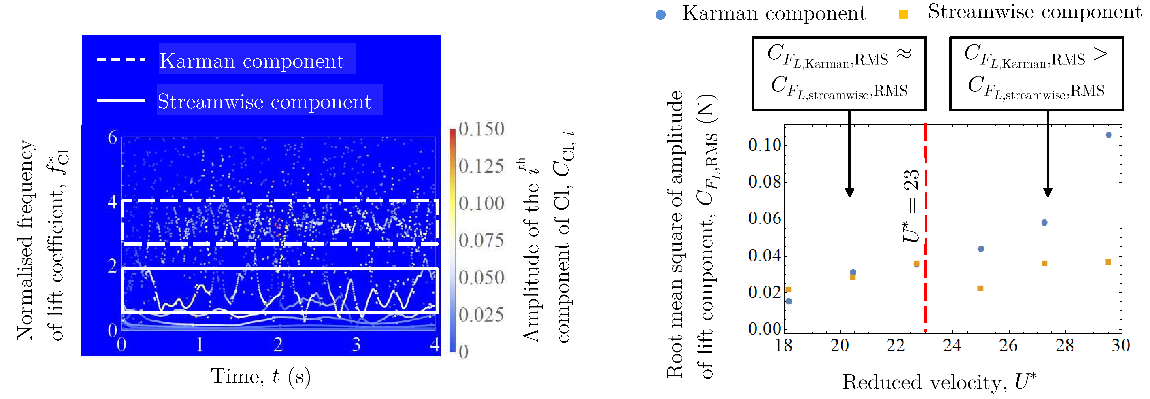
\includegraphics[width=1\textwidth]{figs/graphicalAbstract}
\end{graphicalabstract}
% >>>

% Highlights <<<
\begin{highlights}
\item Two main vibration regimes exist in a pure cruciform energy harvester
\item Alternating lift due to Karman and streamwise vortex exist in superposition
\item Streamwise vortex disrupts the periodicity and self-similarity of alternating lift
\item Power output can increase by reducing energy lost to production of Karman vortex
\end{highlights}
% >>>

% Keywords <<<
\begin{keywords}
  Vortex-induced vibration \sep Vibration energy harvester \sep CFD simulation \sep Streamwise vorticity \sep Ensemble empirical mode decomposition (EEMD) \sep Hilbert transform
\end{keywords}
% >>>

% Make title and set spacing <<<
\maketitle

\doublespacing
% >>>

\section{Introduction} \label{sec:intro}
Streamwise vortex-induced vibration (SVIV) is a type of vortex-induced vibration (VIV) driven by vortical structures whose vorticity vector points in the direction of the free stream. In recent decades, there have been efforts to exploit the SVIV phenomenon from cruciform structures for energy harvesting, an example of which is given in Fig. \ref{fig:cruciformSystemSchematic}. The literature on this subject can be broadly categorised into two groups: how the mechanical properties of the oscillator (e.g., mass ratio, damping, etc.) affects the amplitude/frequency response of SVIV \citep{Koide2009,Koide2013,Nguyen2012} and how the minutiae of the flow field affect the force driving the vibration of the cylinder, i.e. the fluid mechanical aspect of the system \citep{Deng2007,Koide2017,Zhao2018a}.

In the first focus area, researchers studied some permutation of the following method to convert the vibration into electrical power. The method consists of a coil and magnet. The coil, which moves with the vibrating cylinder, creates relative motion against the magnet, which is placed in the hollow of the coil \citep{Koide2009}. While investigating the system at a Reynolds number in the order of $\re \sim O \left( 10^{4} \right)$, \citet{Koide2009} showed that increased damping due to energy harvesting reduces the maximum vibration amplitude close to a factor of 4. Amplitude reduction due to increased total damping was also mentioned in \citet{Bernitsas2008a,Bernitsas2008b,Bernitsas2009}. Further investigation in \citet{Nguyen2012} revealed that damping not only affects the amplitude response of the cylinder but also narrows the synchronisation region between vortex shedding and cylinder vibration. Moreover, \citet{Nguyen2012} demonstrated a strong coupling between mass ratio and damping in determining both the width of the synchronisation region and the maximum amplitude response of the cylinder.

In the second focus area, investigators turned their attention to the details of the flow where streamwise vortex shedding occurs. One such study carefully shot motion pictures of the dye-injected flow \citep{Koide2017} at Reynolds number in the order of $\re \sim O\left( 10^{3} \right)$. A lower Reynolds number (Re) reduces the amount of turbulence in the flow, allowing a clearer shot of the vortex structures. Their study also highlights the higher level of turbulence produced by the circular cylinder-strip plate cruciform in contrast to the twin circular cylinder cruciform, which diminishes the periodicity of vortex shedding. Although visually enlightening, this and other more qualitative studies contribute little towards improving our understanding of the relationship between vortex shedding and the resulting lift. \citet{Deng2007} demonstrated a way to overcome such a shortcoming.

In their study, \citet{Deng2007} examined the flow field of a twin circular cylinder cruciform using computational fluid dynamics (CFD). Their domain stretches  $28D$  in the streamwise direction,  $16D$  in the transverse direction and  $12D$  in the spanwise direction. They studied an Re range yet another order of magnitude smaller than that studied by \citet{Koide2017}, possibly to get an even clearer visualisation of the vortical structures with less turbulence, and to ease computational requisites. At a fixed  $\re = 150$ , streamwise vortices form even at a gap ratio of $2$. This result differs quite strikingly from \citet{Koide2006,Koide2007}, conducted at an Re twice the order of magnitude of \citet{Deng2007}, an indication that the minimum gap ratio needed for the onset of streamwise varies with respect to Re.

They also observed that when the gap ratio $G$, which they denote as  $L/D$  in their paper, increases from 3 to 4, the maximum amplitude of the lift coefficient increases by almost threefold. This can be attributed quite easily to the current vortex pair shed by the upstream cylinder. The downstream cylinder immediately disturbs the pair shed from the upstream cylinder when  $G=3$. The lift coefficient increases by about a factor of 3 when this immediate disturbance diminishes at  $G=4$. The visualisation of three-dimensional (3D) vorticity isocontours enables us to quickly establish this link vis-\`{a}-vis the lift coefficient signal. The authors use of CFD made this possible.

A similar study in the order of magnitude $\re \sim O \left( 10^{2} \right)$ by \citet{Zhao2018a} particularly highlighted the immense utility of CFD as a tool to research SVIV or flow around a cruciform in general. They computed the sectional lift coefficient along the upstream cylinder, and the time history of this sectional lift coefficient revealed two different modes of vortex shedding, namely, parallel and K-shaped. They also paid attention to the local flow patterns that vary along the length of the upstream cylinder such as the trailing vortex flow, necklace vortex flow and flow in the small gap (denoted as SG flow). The discontinuities in the phase angle of the sectional lift coefficient along the upstream cylinder seems to suggest the inadequateness of attributing the lift coefficient to streamwise vortex shedding alone, particularly when Karman vortex streamlines were also observed some distance away from the junction of the cruciform. \citet{Shirakashi1989} also made a similar observation in their experimental work. This leads us to hypothesise that the lift signal is more appropriately viewed as the streamwise-Karman vortex-induced composite lift signal. However, we could not find studies that took this viewpoint and worked out its implication on power generation in their investigation of SVIV.

The objectives of this study are thus threefold: (1) to take a closer look at the amplitude and frequency response of a circular cylinder-strip plate cruciform, especially in reduced velocity ($\ured$) ranges where the transition from KVIV to SVIV occurs, (2) to demonstrate the compositeness of the lift signal of an SVIV system and establish the difference between the lift signal characteristics in the KVIV and SVIV regime and (3) to shed light on how the contribution from the Karman and streamwise components of lift changes as we increase $\ured$ after the onset of SVIV and predict how much improvement in the power generation can be anticipated if we are able to unify the lift amplitude contributions due to Karman and streamwise vortex shedding. Here, $\ured = U/\fn D$, with $U$, $\fn$ and $D$ being the freestream velocity, natural frequency of the system and the diameter of the circular cylinder respectively. The following \S\ref{sec:method} details the methodology we employ to conduct this study. We present and discuss our results in \S\ref{sec:singPlateResp}, \S\ref{sec:tempEvo}, and \S\ref{sec:estimPow}. We describe our conclusions in \S\ref{sec:conclusions}.

\begin{figure}
  \centering
  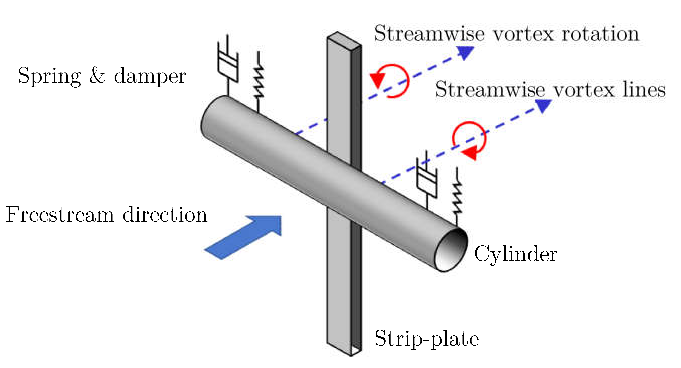
\includegraphics[width=0.5\textwidth]{figs/figure1}
  \caption{A schematic of the circular cylinder-strip plate cruciform system. Alternate shedding of the streamwise vortices create the alternating lift that drives the vibration of the cylinder.}
  \label{fig:cruciformSystemSchematic}
\end{figure}


\section{Methodology} \label{sec:method}
\subsection{Problem geometry} \label{ssec:probGeo}
The geometrical setup for this study builds on the work of \citet{Maruai2017,Maruai2018} who studied both experimentally and numerically the \textcolor{blue}{flow-induced motion} (FIM) of a square cylinder with a downstream flat plate. Their simulation results are in good agreement with their own experiment, and with the experimental results of \citet{Kawabata2013}, in the Reynolds number range $3.6\times10^{3}<\text{Re}<12.5\times10^{3}$. This is well within the Reynolds number studied in this work, i.e. $1.1\times10^{3}<\text{Re}<14.6\times10^{3}$.

Our $x-y$ plane fundamentally follows the dimensions used in \citet{Maruai2017,Maruai2018}, except for the cylinder shape, which in this study is circular, and the $20D$ distance to the outlet is measured from the downstream face of the strip-plate. This is shown in Fig. \ref{fig:problemGeometry}. We chose the cylinder-plate gap $G$ to be $0.16D$, as \citet{Koide2013} has shown that this gap size sustains the highest SVIV amplitude over the widest range of $\ured$, in comparison to other gap sizes.

\begin{figure}
  \centering
  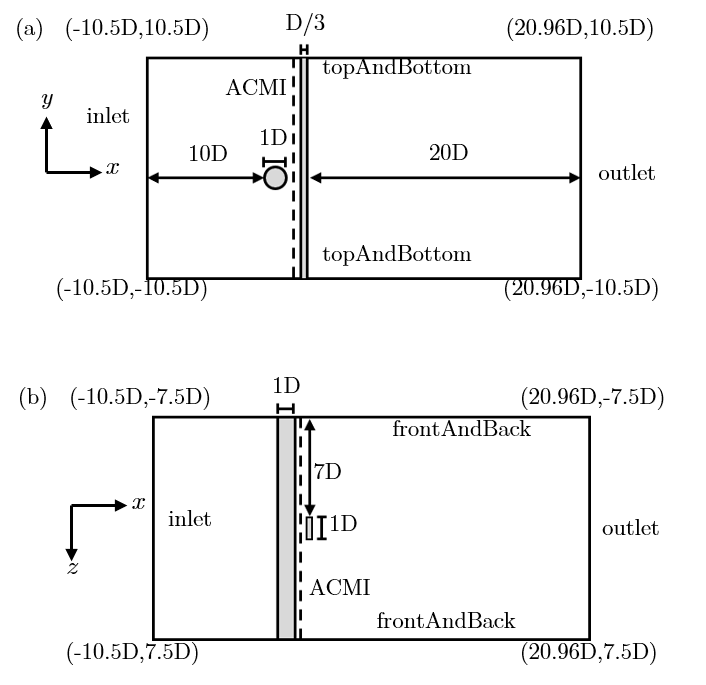
\includegraphics[width=0.5\textwidth]{figs/figure2}
  \caption{Problem geometry and coordinate system used. Figure \ref{fig:problemGeometry}a shows the side view of the simulation domain (cross-section perpendicular to the freestream) while Fig. \ref{fig:problemGeometry}b shows the top view of the simulation domain (cross-section parallel to the freestream). Note that the gap ratio $G$ between the cylinder and the strip plate is $0.16D$, and the arbitrarily coupled mesh interface (ACMI) patch is located midway through the gap, i.e., $0.08D$ downstream from the trailing edge of the cylinder.}
  \label{fig:problemGeometry}
\end{figure}

As the problem geometry is explicitly three-dimensional (3D), the $x-y$ plane is extruded in the $z$ direction, thus obtaining a 3D domain. As can be seen in Fig. \ref{fig:problemGeometry}, the circular cylinder extends from $z/D=7.5$ to $z/D=-7.5$, while the strip-plate extends from $-10.5$ to $y/D=10.5$. The $z-$direction extent is set as $z/D=\pm7.5$ is already more than twice the spanwise reach of the streamwise vortex, thus sufficient for the vortices to materialise in our numerical solution. To compare, the spanwise extent of the numerical study by \citet{Deng2007}, is $z/D=\pm6$ and the spanwise extents of experiments by \citet{Nguyen2012} and \citet{Koide2013} are $z/D=\pm5$.

\color{blue}
Table \ref{tab:boundConds} summarises the boundary conditions imposed on each of the boundary patches in the simulation domain (see Fig. \ref{fig:convergenceStudy}). The symbols $U$, $p$, $\nut$, and $\nuTilda$ refer to the flow velocity, pressure, kinetic eddy viscosity and its mediating variable, respectively. At the inlet, the \verb|fixedValue| for $U$ is the freestream velocity $U_{\infty}$ (\si[per-mode=symbol]{\metre\per\second}), while $U = \SI[per-mode=symbol]{0}{\metre\per\second}$ at the strip plate. The \verb|fixedValue| for $p$ at the outlet is \SI[per-mode=symbol]{0}{\square\metre\per\square\second}, and the \verb|fixedValue| for $\nuTilda$ is \SI[per-mode=symbol]{0}{\square\metre\per\second} at the cylinder and strip plate patches.

\begin{table}[width=1\linewidth,cols=5,pos=h]
  \color{blue}
  \caption{Boundary conditions imposed on each boundary patch of the computational domain.} \label{tab:boundConds}
\begin{tabular*}{\tblwidth}{@{} LLLLL@{} }
\toprule
Patch / Flow parameter  & $U$                       & $p$                       & $\nut$                          & $\nuTilda$        \\
\midrule
Inlet                   & \verb|fixedValue|         & \verb|zeroGradient|       & \verb|freestream|               & \verb|freestream| \\
Outlet (opposite Inlet) & \verb|zeroGradient|       & \verb|fixedValue|         & \verb|freestream|               & \verb|freestream| \\
Top                     & \verb|freestream|         & \verb|freestreamPressure| & \verb|freestream|               & \verb|freestream| \\
Bottom (opposite Top)   & \verb|freestream|         & \verb|freestreamPressure| & \verb|freestream|               & \verb|freestream| \\
Front                   & \verb|freestream|         & \verb|freestreamPressure| & \verb|freestream|               & \verb|freestream| \\
Back (opposite Front)   & \verb|freestream|         & \verb|freestreamPressure| & \verb|freestream|               & \verb|freestream| \\
Cylinder                & \verb|movingWallVelocity| & \verb|zeroGradient|       & \verb|nutUSpaldingWallFunction| & \verb|fixedValue| \\
Strip plate             & \verb|fixedValue|         & \verb|zeroGradient|       & \verb|nutUSpaldingWallFunction| & \verb|fixedValue| \\
\bottomrule
\end{tabular*}
\end{table}
\color{black}

\subsection{Numerical method} \label{ssec:numMeth}
The objectives of our study necessitate the solution of the continuity, and 3D unsteady Reynolds averaged Navier-Stokes (3D URANS) equations. We achieve this by using OpenFOAM, an open-source computational fluid dynamics (CFD) platform written in C++. Specifically, we work to solve the following continuity and URANS equations.

\begin{equation}
  \frac{\partial U_{i}}{\partial x_{i}}=0,
  \label{eq:continuity}
\end{equation}

\begin{equation}
  \frac{\partial U_{i}}{\partial t}+U_{j}\frac{\partial U_{i}}{\partial x_{j}} = -\frac{1}{p}\frac{P}{x_{i}}+\frac{\partial}{\partial x_{j}} \left( 2\nu S_{ij}-\overline{u'_{j}u'_{i}} \right).
  \label{eq:navier-stokes}
\end{equation}

The symbols $U$, $x$, $t$, $\rho$, $P$, $\nu$, $S$, and $u'$ are the mean component of velocity, spatial component, time, density, pressure, kinematic viscosity, mean strain rate and the fluctuating component of velocity, respectively. The mean strain rate $S_{ij}$ is given by

\begin{equation}
  S_{ij} = \frac{1}{2} \left( \frac{\partial U_{i}}{\partial x_{j}} + \frac{\partial U_{j}}{\partial x_{i}} \right).
  \label{eq:sij}
\end{equation}

This study employs the Spalart-Allmaras turbulence model to approximate the Reynolds stress tensor $\tau_{ij} = \overline{u'_{j}u'{i}}$. This turbulence model has been shown to produce results that agree reasonably well with experiments in similar flow-induced motion (FIM) studies \citep{Ding2015a,Ding2015b}. We use the Boussinesq approximation to relate the Reynolds stress tensor to the mean velocity gradient

\begin{equation}
  \tau_{ij} = 2 \nu_{T}S_{ij},
  \label{eq:tauij}
\end{equation}

\noindent where $\nu_{T}$ represents the kinetic eddy viscosity. $\nu_{T}$ is, in turn, a function of $\tilde{\nu}$ and $f_{\nu 1}$, while $f_{\nu 1}$ is a function of $\chi$ and $c_{\nu 1}$, and $\chi$ a function of $\tilde{\nu}$ and $\nu$, as shown in Eq. \ref{eq:kineticeddy}.

\begin{subequations}
  \label{eq:kineticeddy}
  \begin{align}
    \nu_{T}   & = \tilde{\nu} f_{\nu 1}, \label{eq:kineticeddyA}\\
    f_{\nu 1} & = \frac{\chi^{3}}{\chi^{3}+c^{3}_{\nu 1}}, \label{eq:kineticeddyB}\\
    \chi      & = \frac{\tilde{\nu}}{\nu}. \label{eq:kineticeddyC}
\end{align}
\end{subequations}

\noindent Here, $\tilde{\nu}$ serves to mediate the turbulence model and dictates how $\tilde{\nu}$ is conserved.

\begin{align}
  \label{eq:kineticEddyTransport}
  \frac{\partial \tilde{\nu}}{\partial t} &+ U_{j} \frac{\partial \tilde{\nu}}{\partial x_{j}} = c_{b1}\tilde{S}\tilde{\nu} - c_{w1} f_{w} \left( \frac{\tilde{\nu}}{D} \right)^{2} \nonumber \\
  &\qquad {} + \frac{1}{\sigma} \left\{ \frac{\partial}{\partial x_{j}} \left[ \left( \nu + \tilde{\nu} \right) \frac{\partial \tilde{\nu}}{\partial x_{j}} \right] c_{b2} \frac{\partial \tilde{\nu}}{\partial x_{i}} \frac{\partial \tilde{\nu}}{\partial x_{i}} \right\}
\end{align}

$c_{b1}$, $c_{b2}$, and $c_{\nu 1}$ are constant with values $0.1335$, $0.622$ and $7.1$ respectively. $c_{w1}$ is given by

\begin{equation}
  c_{w1} = \frac{c_{b1}}{\kappa} + \frac{1+c_{b2}}{\sigma},
  \label{eq:cw1}
\end{equation}

\noindent where additional constants $\kappa$ and $\sigma$ are $0.41$ and $2/3$ respectively. $f_{w}$, on the other hand, is given by

\begin{equation}
  f_{w} = g \left( \frac{1 + c^{6}_{w3}}{g^{6} + c_{w3}} \right)^{\frac{1}{6}}.
  \label{eq:fw}
\end{equation}

\noindent Here, $c_{w3} = 2$ while $g$ is given by

\begin{equation}
  g = r + c_{w2} \left( r^{6} - r \right),
  \label{eq:g}
\end{equation}

\noindent where $r$ is

\begin{equation}
  r = \text{min} \left( \frac{\tilde{\nu}}{\tilde{S} \kappa^{2} d^{2}}, 10 \right),
  \label{eq:r}
\end{equation}

Additionally, $\tilde{S}$ is

\begin{equation}
  \tilde{S} = \Omega + \frac{\tilde{\nu}}{\kappa^{2} d^{2}} f_{\nu 2},
  \label{eq:sTilde}
\end{equation}

\noindent where $\Omega$ and $d$ are the magnitude of vorticity and the distance from the mesh nodes to the nearest wall, respectively. Finally, $f_{\nu 2}$ is

\begin{equation}
  f_{\nu 2} = 1 - \frac{\chi}{1 + \chi f_{\nu 1}}.
  \label{eq:fv2}
\end{equation}

\noindent We solve these equations numerically using the PIMPLE algorithm, which combines the transient solver PISO with the steady-state solver SIMPLE for improved numerical stability.

\subsection{Dynamic mesh motion} \label{ssec:dynMesh}

In this study, the cylinder in VIV moves perpendicular to the free stream direction. The motion unavoidably distorts the mesh around it, degrading important mesh metrics such as non-orthogonality and skewness. However, we can diffuse the mesh deformation to the neighbouring nodes as per the following Laplace equation,

\begin{equation}
  \nabla \cdot \left( \gamma \nabla u \right) = 0.
  \label{eq:laplace}
\end{equation}

\noindent Here, $u$ represents the mesh deformation velocity and $\gamma$ is displacement diffusion. We chose $\gamma = 1/l^{2}$, where $l$ is the cell centre distance to the nearest cylinder edges. We implement the GAMG linear solver with the Gauss-Seidel smoother to solve Eq. \ref{eq:laplace}. The dynamic mesh algorithm then updates the mesh node positions according to the following equation.

\begin{equation}
  x_{\text{new}} = x_{\text{old}} + u \Delta t
  \label{eq:meshNodeUpdate}
\end{equation}

\noindent The solver resumes the solution of Eqs. \ref{eq:continuity} and \ref{eq:navier-stokes} once the mesh node positions are updated.

Another dynamic mesh handling technique used in this study is the arbitrarily coupled mesh interface (ACMI) that allows non-conforming meshes to slide over another, thus preserving the mesh quality around a moving object. The tiny gap between the cylinder and strip-plate, limits our ability to diffuse the mesh deformation to the surrounding space. ACMI is thus implemented at the centre of the gap between the circular cylinder and the strip-plate, as shown in Fig. \ref{fig:problemGeometry}, to circumvent this problem. This method has been successfully implemented in the works of \citet{Ding2015b,Zhang2018}, preserving the quality of their mesh and controlling their Courant-Friedrichs-Lewy (CFL) number.

\subsection{Open flow channel experiment} \label{ssec:openFlowExp}
We set up an experimental rig to validate our numerical results at reduced velocity $\ured = 22.7$. We chose $\ured = 22.7$ because that value of $\ured$ is where the vibration-driving mechanism is known to transit from Karman to streamwise vortex shedding \citep{Koide2013}. The experimental rig consists of a closed-loop open channel circuit based on the water tunnel used by \citet{Nguyen2012}, shown in Fig. \ref{fig:experimentalSetup}. The cross-section of our test section is a square with sides $100$ mm in length. The test section is $1500$ mm long.

\begin{figure}
  \centering
  \begin{subfigure}[h]{0.5\textwidth}
    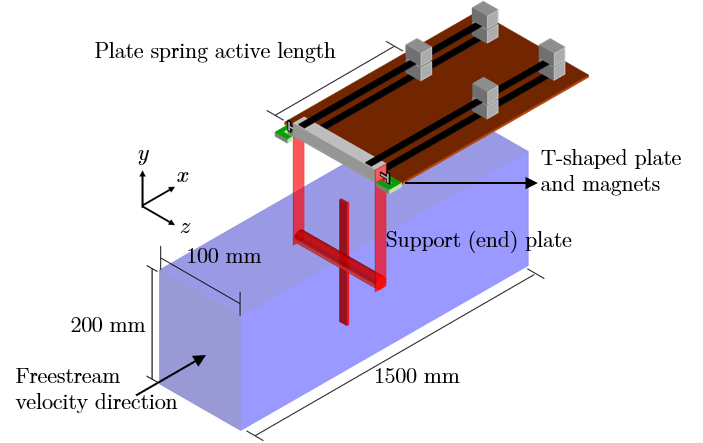
\includegraphics[width=\textwidth]{figs/figure3a}
    \caption{}
    \label{fig:rigSketch}
  \end{subfigure}

  \begin{subfigure}[h]{0.35\textwidth}
    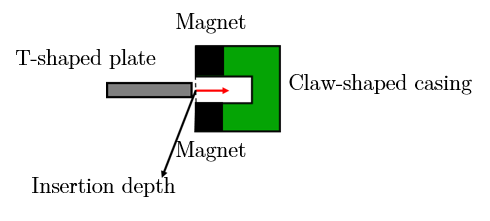
\includegraphics[width=\textwidth]{figs/figure3b}
    \caption{}
    \label{fig:damperSketch}
  \end{subfigure}

  \caption{A schematic of our experimental setup. Figure \ref{fig:rigSketch} presents a 3D schematic of the experimental rig while Fig. \ref{fig:damperSketch} shows an enlarged schematic of the damping system.} \label{fig:experimentalSetup}
\end{figure}

The system for providing elastic support and damping to the circular cylinder follows closely those used by \citet{Kawabata2013} and \citet{Koide2013,Koide2017}, which can be summarised as follows. The stiffness coefficient $k$ of the plate spring is determined through a simple weight versus displacement test \citep{Sun2016}, at various active lengths of the spring. This provides a calibration curve of stiffness coefficient, $k$ against plate spring length, $l$. We can then adjust the length of the plate spring to obtain the desired value for $k$.

On the other hand, the damping of the system is adjusted using T-shaped aluminium plates fixed at either end of the cylinder endplate, and a pair of neodymium magnets contained in a claw-shaped casing. The further the T-shaped plate is pushed into the opening of the claw, the denser the magnetic field it needs to cut through during motion, thus dissipating more energy. We then calibrate the damping produced at various depths at which the T-shaped plate is pushed into the casing, via free-decay tests of the cylinder in still water. The procedure for conducting free-decay tests are detailed in \citet{Raghavan2007}.

Flow inside the open channel is driven by a $3.728$ kW (5 hp) centrifugal pump, controlled using a voltage controller. The input voltage for the centrifugal pump is calibrated against the centreline velocity of the test section, $750$ mm from the inlet, i.e. mid-length of the test section. We show this schematically in Fig. \ref{fig:keyDimensions}. Here, we define the centreline of the test section as the line $50$ mm from the bottom and $50$ mm from either of the sidewalls of the test section. We placed the cylinder in the same position during experimental runs. The centreline velocity $U_{\text{cent.}}$ is measured using an acoustic Doppler velocimeter (ADV), sampling at $200$ Hz. The resulting calibration curve is applicable for determining $U_{\text{cent.}}$ at input voltages $30 < V_{\text{in}} \text{(V)} < 100$. We measured the turbulence intensity along the centreline to be about $5\%$.

We obtained the time history for cylinder displacement, $y$, by using a video camera pointed normal to the cylinder endplate. We placed a visual marker on the endplate, and the motion of the marker captured by the camera is analysed using \textit{Tracker}: a motion analysis tool built on the Open Source Physics Java framework. To validate our experimental setup, we tuned to the best of our ability our experimental parameters to the values used by \citet{Koide2013} and test whether we can replicate their results. Table \ref{tab:expParameter} summarises the parameters in lieu of that paper.


\begin{figure}
  \centering
  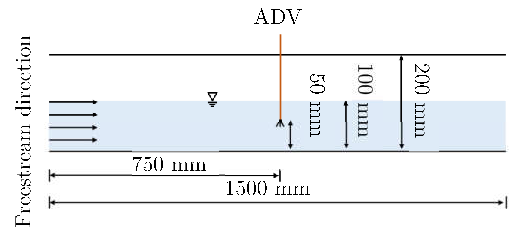
\includegraphics[width=0.4\textwidth]{figs/figure4}
  \caption{Side view of the open flow channel, in schematic form. Also, key dimensions of the experimental setup. The acoustic Doppler velocimeter (ADV) is placed at the same location where the cylinder is located during experimental runs.}
  \label{fig:keyDimensions}
\end{figure}

\begin{table}[width=0.9\linewidth,cols=3,pos=h]
  \caption{Summary of experimental parameters in contrast to those used in the experimental work of \citet{Koide2013}.} \label{tab:expParameter}
\begin{tabular*}{\tblwidth}{@{} LLL@{} }
\toprule
                                           & Current study & \citet{Koide2013}\\
\midrule
Cylinder diameter, $D$ (m)                 & $0.01$        & $0.01$           \\
Cylinder length, $l_{\text{cylinder}}$ (m) & $0.09$        & $0.098$          \\
Strip-plate width (m)                      & $0.01$        & $0.01$           \\
Strip-plate length (m)                     & $0.1$         & $0.1$            \\
Effective mass, $m_{\text{eff.}}$ (kg)     & $0.162$       & $0.174$          \\
Logarithmic damping, $\delta$              & $0.178$       & $0.24$           \\
Scruton number, Sc                         & $9.94$        & $7.74$           \\
System natural frequency, $f_{n}$ (Hz)     & $4.42$        & $4.4$ to $4.79$  \\
\bottomrule
\end{tabular*}
\end{table}

We show a sample of the normalised displacement -- $\ystr = y/D$ -- time series in Fig. \ref{fig:sampTimeHist}. Computing the statistics of $\ystr$ and the normalised cylinder vibration frequency, $\fstr = \fcyl/\fn$ ($\fcyl$ being the vibration frequency of the cylinder), from several runs gave us a value of $\ystr = 0.33 \pm 0.03$ and $\fstr = 1.03 \pm 0.04$. \citet{Koide2013} obtained $\ystr = 0.32$  and $\fstr = 1.09$ under a similar $\ured$ condition. We thus take this fairly successful reproduction of the results of \citet{Koide2013} as an indication of readiness for further data collection.

\begin{figure}
  \centering
  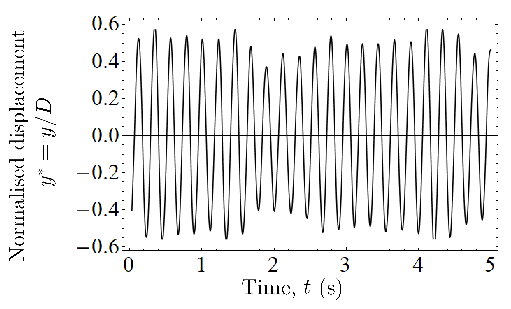
\includegraphics[width=0.41\textwidth]{figs/figure5}
  \caption{A sample of the time history for cylinder displacement from a test run of our experimental setup. The value of reduced velocity is $\ured = 22.7$.}
  \label{fig:sampTimeHist}
\end{figure}


\section{Numerical setup validation} \label{sec:numSetup}
\subsection{Grid independency study via Richardson extrapolation and grid convergence index} \label{ssec:richExtrap}
\textcolor{blue}{A common method for checking the grid independency of quantities of interest in a numerical study is by demonstrating that one obtained similar results on all variants of the spatial discretisation (usually three grids), and then proceeding with the numerical study using the medium variant on the computational domain (see, e.g., \citet{Ding2013}, \citet{Ding2019}, or \citet{Wang2020}, which settled on the coarse variant of their spatial discretisation).} Our method of choice however, checks for the convergence of the quantities of interest as one solves the governing equation on successively finer grid resolutions \citep{Richardson1927,Stern2001}. This method pays attention not only on the presumed converged value, but also on the trend of convergence. Literature that employ this method impose a monotonic convergence condition \citep{Stern2001,MatAli2011,Ali2012,Maruai2018} on their quantities of interest, adding an extra layer of confidence in the final form of the spatial discretisation.

Additionally, this method allows for a quantitative description of the degree of convergence through the grid convergence index (GCI). Let $f_{1},f_{2},f_{3},\dots,\fk$ denote the quantity of interest obtained from several grids. A larger subscript indicates a coarser grid, thus, $f_{1}$ denotes the finest while $\fk$ denotes the coarsest grid. Let the difference between successive solutions be $\epsilon_{2,1},\epsilon_{3,2},\epsilon_{4,3},\dots,\epsilon_{n,n-1}$, where $\epsilon_{2,1} = f_{2} - f_{1}$, $\epsilon_{3,2} = f_{3} - f_{2}$ and so on. Then, the GCI is defined as

\begin{equation}
  \text{GCI}_{i+1,i} = F_{s} \frac{\left |\epsilon_{i+1,i} \right |}{f_{i} \left ( r^{p} - 1 \right )} \times 100\%,
  \label{eq:gci}
\end{equation}

\noindent where $F_{s}$, $f_{i}$ and $r^{p}$ denotes the safety factor $\left ( = 1.25 \right )$, quantity of interest and the refinement ratio, $r$, between successive grids raised to the order of accuracy of the series of solution, $p$. We refer the reader to \citet{Stern2001,Langley2018} for a more detailed discussion on $r^{p}$.

We can estimate what the solution approaches as the grid size approaches zero by using the $\text{p}^{\text{th}}$ method. Briefly, we compute the generalised Richardson extrapolation of the quantity of interest as follows.

\begin{equation}
  \fre = f_{1} + \frac{f_{1} - f_{2}}{\rp - 1},
  \label{eq:richardsonExtrapolation}
\end{equation}

\noindent where $\fre$ is the Richardson extrapolation of the quantity of interest. Using $\fre$ to estimate the limit of the monotonically convergent series of $f_{i}$, we can determine the percentage difference of our solution on our finest grid from this limit as

\begin{equation}
  E_{i} = \frac{f_{i} - \fre}{\fre} \times 100\%.
  \label{eq:percentageDifference}
\end{equation}

Table \ref{tab:gridIndependency} summarises the result of our grid independency study for the SVIV reduced velocity of $\ured = 22.7$. We identified three quantities central to the investigation of fluid-structure phenomena, especially the flow-induced vibration of a circular cylinder. They are the vibration amplitude, vibration frequency and lift coefficient of the cylinder. We solve the governing equations on three grids which are numbered $1$ for the finest, $2$ for the medium and $3$ for the coarsest, shown in Fig. \ref{fig:convergenceStudy}. If we let $v_{i}$ be the volume of the $i^{\text{th}}$ cell in the grid and $N$ be the total number of cells in the domain, then, the average cell size is

\begin{figure}
  \centering
  \begin{subfigure}[h]{0.3\textwidth}
    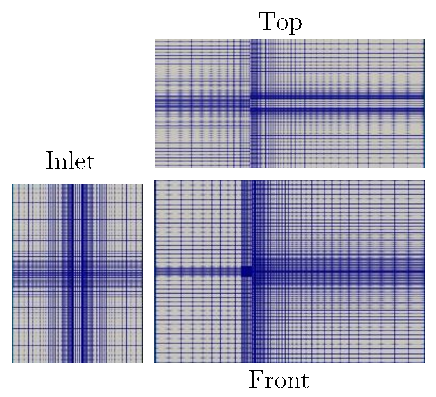
\includegraphics[width=\textwidth]{figs/figure6a}
    \caption{Coarse}
    \label{fig:coarseMesh}
  \end{subfigure}

  \begin{subfigure}[h]{0.3\textwidth}
    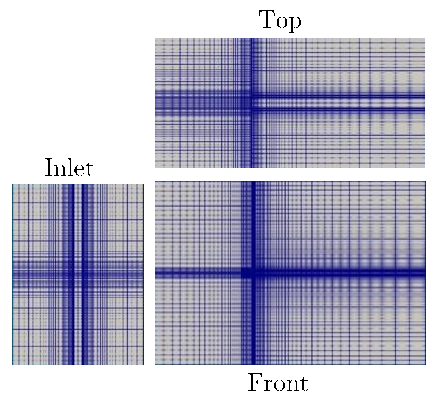
\includegraphics[width=\textwidth]{figs/figure6b}
    \caption{Medium}
    \label{fig:mediumMesh}
  \end{subfigure}

  \begin{subfigure}[h]{0.3\textwidth}
    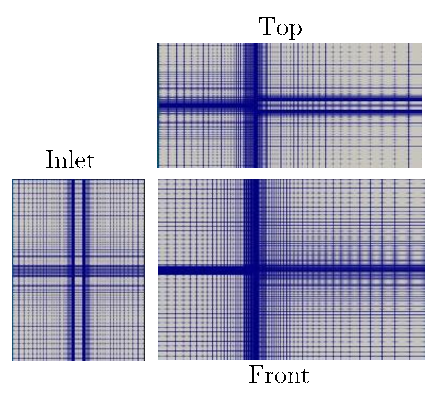
\includegraphics[width=\textwidth]{figs/figure6c}
    \caption{Fine}
    \label{fig:fineMesh}
  \end{subfigure}

  \caption{Three meshes used in the grid convergence study. Figures \ref{fig:coarseMesh}, \ref{fig:mediumMesh} and \ref{fig:fineMesh} show the coarse, medium and fine meshes viewed perpendicular to three main viewing positions: from the inlet, the top and the front, which is looking directly at the cylinder end.} \label{fig:convergenceStudy}
\end{figure}

\begin{equation}
  h = \frac{1}{N} \left [ \sum_{i=1}^{N} v_{i} \right ]^{1/3},
  \label{eq:averageCellSize}
\end{equation}

\noindent and the normalised average cell size is hence 


\begin{equation}
  h/D = \frac{1}{ND} \left [ \sum_{i=1}^{N} v_{i} \right ]^{1/3}.
  \label{eq:normAveCellSize}
\end{equation}

Both $\yrms$ and $\clrms$ starts at an initial value smaller than their Richardson extrapolations, $\fre$, before approaching it as we decrease the average cell size, $h$. This similar trend can perhaps be attributed to the causal relationship between the lift coefficient and vibration amplitude. The lift drives and sustains the vibration, hence a small lift produces a small vibration, and when the lift amplitude becomes higher, so too does the vibration amplitude. The vibration frequency, on the other hand, starts at a value larger than its $\fre$ before approaching $\fre$.

The quantity $\clrms$ experiences the most significant drop in GCI as we refine the grid. The GCI is close to one-third $\left ( 30.92\% \right )$ as we refine the grid from coarse to medium with a refinement ratio of $1.376$. The refinement ratio is calculated by dividing the number of cells in one grid with the next one down the refinement line. Following the grid numbering convention explained previously, dividing the number of cells in the fine grid (grid 1) with the number of cells in the medium grid (grid 2) gives us the refinement ratio from medium to fine, or $r_{2,1}$. Similarly, dividing the number of cells in the medium grid (grid 2) with the number of cells in the coarse grid (grid 3) gives us the refinement ratio from coarse to medium, or $r_{3,2}$. We can generalise this to $i-$number of grids as follows.

\begin{equation}
  r_{i+1,i} = \frac{S_{\text{grid},i+1}}{S_{\text{grid},i}},
  \label{eq:refinementRatio}
\end{equation}

\noindent where $S_{\text{grid},i}$ denotes the total number of cells in the $i^{\text{th}}$ grid. The GCI of $\clrms$ drops further to $1.63\%$ as the mesh is refined more with a refinement ratio of $1.304$.

The GCI for $\yrms$ also drops by one order of magnitude as can be seen by comparing $\text{GCI}_{3,2}$ with $\text{GCI}_{2,1}$. Again, this similar trend of improvement points to the causal relationship between lift and displacement of the cylinder. The GCI for $\fstr$, however, drops by approximately a factor of $6$ instead of one order of magnitude, unlike the GCIs of $\yrms$ and $\clrms$.

\begin{table}[width=0.9\linewidth,cols=4,pos=h]
  \caption{Summary of grid independency study.} \label{tab:gridIndependency}
\begin{tabular*}{\tblwidth}{@{} LLLL@{} }
\toprule
Parameter/ metric                                                       & $\clrms$       & $\yrms = \ystr/D$ & $\fstr = \fcyl / \fn$ \\
\midrule
$\fre$                                                                  & $0.262$        & $0.369$           & $0.969$               \\
$f_{1}$                                                                 & $0.2598$       & $0.3687$          & $0.9695$              \\
$f_{2}$                                                                 & $0.2430$       & $0.3588$          & $0.9740$              \\
$f_{3}$                                                                 & $0.0805$       & $0.2374$          & $1.0220$              \\
$\left | \epsilon_{2,1} \right |$                                       & $0.02$         & $0.01$            & $0.004$               \\
$\left | \epsilon_{2,1} \right |$                                       & $0.16$         & $0.12$            & $0.48$                \\
$R = \left | \epsilon_{2,1} \right | / \left | \epsilon_{2,1} \right |$ & $0.10$         & $0.08$            & $0.094$               \\
$\text{GCI}_{3,2}$                                                      & $30.92$        & $6.00$            & $0.64$                \\  
$\text{GCI}_{3,2}$                                                      & $1.63$         & $0.52$            & $0.10$                \\
\bottomrule
\end{tabular*}
\end{table}

We provide visual representations of the convergent $\clrms$, $\yrms$ and $\fstr$ series in Figs. \ref{fig:yrmsGCI}, \ref{fig:fstrGCI} and \ref{fig:clrmsGCI}. Note how the quantity of interest is very close to its Richardson extrapolation at the fine grid (grid 1) for all $\clrms$, $\yrms$ and $\fstr$. This implies that the fine grid already provides adequate spatial discretisation for the problem we are studying, and further refinements, while able to nudge our solutions even closer to the limit that is the Richardson extrapolation, may not be optimal in terms of usage of computational resources. Values of $\yrms$ and $\fstr$ at the fine grid already fall within experimental uncertainty as evidenced by our measurement in \S \ref{ssec:openFlowExp} and the work by \citet{Koide2013}. Hence, all succeeding numerical data are gathered from the fine grid.


\begin{figure}
  \centering
  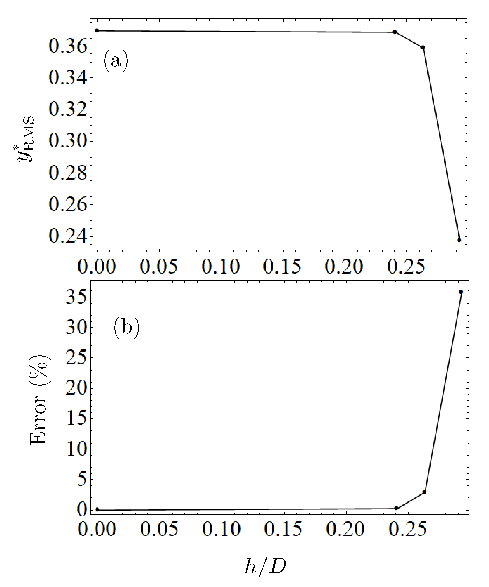
\includegraphics[width=0.39\textwidth]{figs/figure7}
  \caption{The convergence diagram for $\yrms$. Figure \ref{fig:yrmsGCI}a shows how $\yrms$ converges close to the Richardson extrapolation value while Fig. \ref{fig:yrmsGCI}b shows how the error (difference between the value obtained from a particular mesh and the Richardson extrapolation) decreases with decreasing grid spacing.} \label{fig:yrmsGCI}
\end{figure}

\begin{figure}
  \centering
  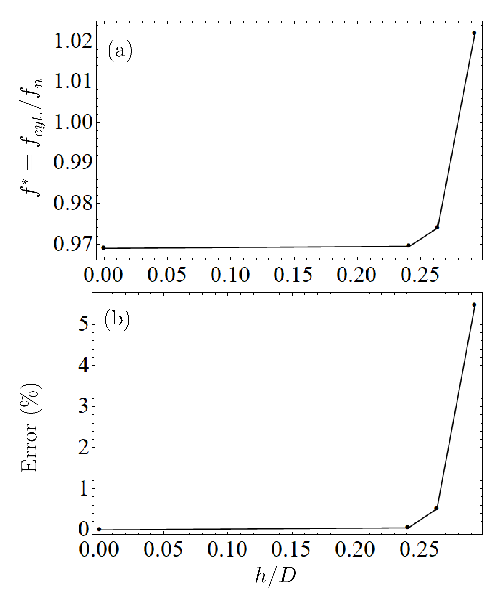
\includegraphics[width=0.4\textwidth]{figs/figure8}
  \caption{The convergence diagram for $\fstr$. Figure \ref{fig:fstrGCI}a shows how $\fstr$ converges close to the Richardson extrapolation value while Fig. \ref{fig:fstrGCI}b shows how the error (difference between the value obtained from a particular mesh and the Richardson extrapolation) decreases with decreasing grid spacing.} \label{fig:fstrGCI}
\end{figure}

\color{blue}
As for the temporal discretisation, we relied on a simple CFL number-based scheme \citep{Hemsuwan2018a,Hemsuwan2018b,Hemsuwan2018c}, in which the time step is chosen such the maximum CFL number $C$ in the computational domain is always less than unity. The CFL number $C$, is defined in Eq. \ref{eq:cflNo} as

\begin{equation}
  C = \frac{U \Delta t}{\Delta x},
  \label{eq:cflNo}
\end{equation}

\noindent where $U$, $\Delta t$ and $\Delta x$ represents the flow velocity, time step and characteristic length of cell, respectively.
\color{black}

\begin{figure}
  \centering
  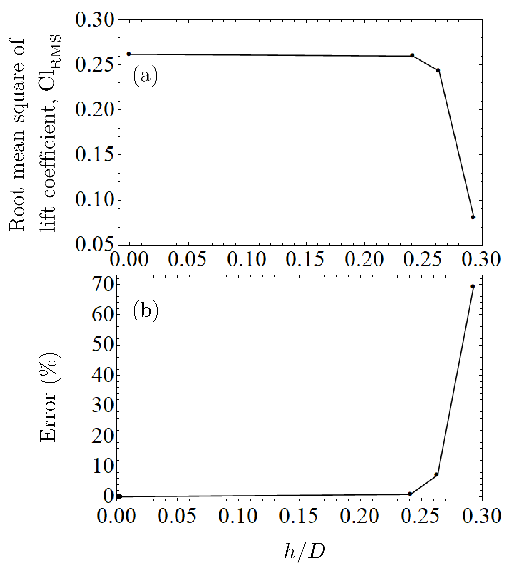
\includegraphics[width=0.43\textwidth]{figs/figure9}
  \caption{The convergence diagram for $\clrms$. Figure \ref{fig:clrmsGCI}a shows how $\clrms$ converges close to the Richardson extrapolation value while Fig. \ref{fig:clrmsGCI}b shows how the error (difference between the value obtained from a particular mesh and the Richardson extrapolation) decreases with decreasing grid spacing.} \label{fig:clrmsGCI}
\end{figure}

\section{Single plate amplitude and frequency response} \label{sec:singPlateResp}
\subsection{Amplitude response} \label{ssec:ampResp}
We compared our experiment and numerical results with those from \citet{Koide2013} and \citet{Nguyen2012} in Fig. \ref{fig:ampFreqComp}. Figure \ref{fig:ampFreqComp}a shows the amplitude response of our single plate experiment and simulation. We use the root-mean-square value of the cylinder displacement to represent the amplitude responses instead of the maximum displacement. The reason for this is twofold: first, using  $\yrms$  facilitates comparison of data with \citet{Nguyen2012} and \citet{Koide2013}, who also used  $\yrms$  in their work. Second, because the cylinder displacement is an intermediate quantity for the estimation of harnessed power \citep{Maruai2017,Maruai2018}, and the usage of root-mean-square amplitude of cylinder displacement gives a direct preview of mean harnessed power.

There is virtually no vibration for both our experiment and simulation when  $\ured \leq \urei$, except for a small peak at $\ured = \urth$. We attribute this peak to the upper branch of KVIV, which still exists, although suppressed due to the cruciform configuration of the system \citep{Shirakashi1989,Nguyen2012}. However, when  $\ured$ exceeds $\urei$, we observe a sudden jump in  $\ured$ right up to about 0.4, for both our experiment and simulation. This we attribute to the formation of the streamwise vortices that drive SVIV.

After the inception of SVIV, the value for  $\yrms$ drops down to approximately 0.3, before recovering to a value that is close to what was observed by \citet{Nguyen2012} and \citet{Koide2013}. This sudden jump followed by a gradual drop and a gradual rise in  $\yrms$ was not found in the works of \citet{Nguyen2012} nor \citet{Koide2013}, even though their experimental parameters are reasonably close to what we use in both our experiment and simulation.


\begin{figure}
  \centering
  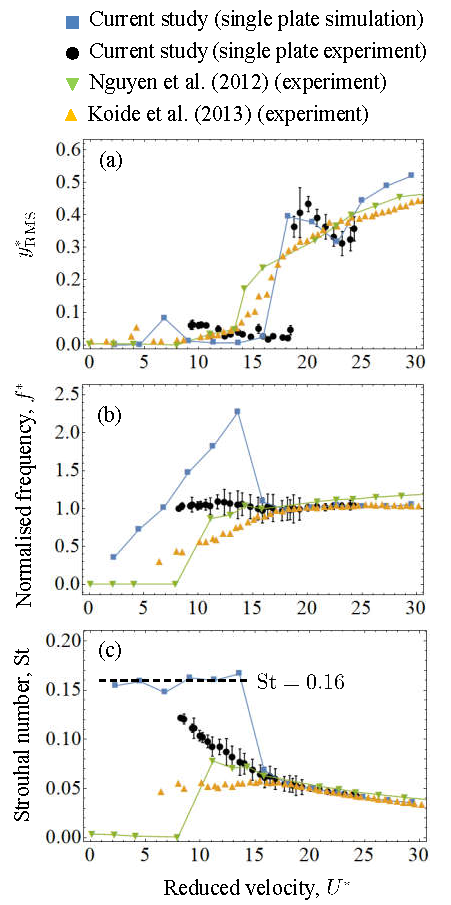
\includegraphics[width=0.4\textwidth]{figs/figure10}
  \caption{The amplitude and frequency response of our cruciform system, compared with results from \citet{Nguyen2012} and \citet{Koide2013}. Figure \ref{fig:ampFreqComp}a shows the amplitude response using $\yrms$, Fig. \ref{fig:ampFreqComp}b the frequency response using $\fstr$ and Fig. \ref{fig:ampFreqComp}c also the frequency response, but using the Strouhal number of vibration.} \label{fig:ampFreqComp}
\end{figure}

We, therefore, attribute this difference to the higher turbulence level set in our work. The turbulence level in the works of \citet{Nguyen2012}, for example, was  $<2.8\%$ throughout their range of Reynolds number. Instead, the initial turbulence level in our setup, both experimental and numerical, is approximately double that value. Because of this, the turbulence amplification due to the onset of streamwise vortices  \citep{Zhao2018a} - especially for a circular cylinder-strip plate cruciform \citep{Koide2017} - is also higher compared to the experiments of \citet{Nguyen2012} and \citet{Koide2013}. This higher compound turbulence warps the dominant vortical structure and introduces an increasing amount of intermittency to the lift signal, and by extension, to the displacement time history of the cylinder. \textcolor{blue}{An intermittent lift signal imposes the same trend on the $\ystr(t)$ signal, reducing its overall mean amplitude, which we compute in this work as $\yrms$.}

One can simply inspect the error bars within  $\urei \leq \ured \leq \urte$ in Fig. \ref{fig:ampFreqComp}a to verify the greater sample dispersion within that range of  $\ured$. This intermittency ultimately vanishes as the dominant vortical structures become sufficiently stable to retain enough periodicity in its formation. Our numerical results also seem to support this argument, as evidenced by the time history of  $\ured$ within $\urei \leq \ured \leq \urtt$ in Fig. \ref{fig:cylDispSignal}. There exists a distinct increase in intermittency for the time histories in Fig. \ref{fig:unstableSVIV}, that disappears once  $\ured \geq 23$ as can be seen in Fig. \ref{fig:stableSVIV}. \textcolor{blue}{We interpret this as the vortical structures becoming more energised and resilient against ambient excitation the further we advance into the SVIV regime.}

\begin{figure}
  \centering
  \begin{subfigure}[h]{0.49\textwidth}
    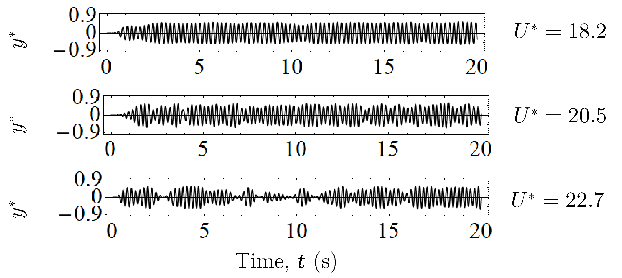
\includegraphics[width=\textwidth]{figs/figure11a}
    \caption{}
    \label{fig:unstableSVIV}
  \end{subfigure}

  \begin{subfigure}[h]{0.49\textwidth}
    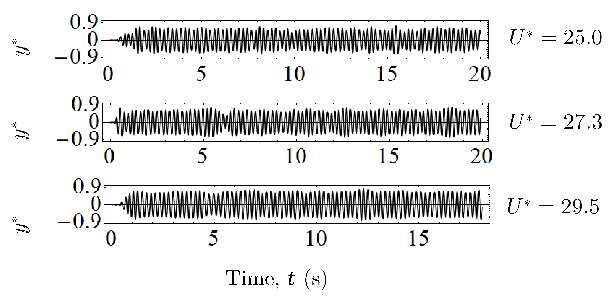
\includegraphics[width=\textwidth]{figs/figure11b}
    \caption{}
    \label{fig:stableSVIV}
  \end{subfigure}

  \caption{The time series of cylinder displacement between $\urei \leq \ured \leq \urtt$. Fig. \ref{fig:unstableSVIV} groups the cylinder displacement signal between $\urei \leq \ured \leq \urte$, where there seems to be an increase in intermittency in the displacement signal, while Fig. \ref{fig:stableSVIV} groups the cylinder displacement signal between $\urel \leq \ured \leq \urtt$, where the intermittency in the displacement signal vanishes.} \label{fig:cylDispSignal}
\end{figure}

\subsection{Frequency response} \label{ssec:freResp}
Figure \ref{fig:ampFreqComp}b compares the frequency responses of our experiment and numerical results with those in \citet{Nguyen2012} and \citet{Koide2013}. We use the normalised frequency  $\fstr$ in Fig. \ref{fig:ampFreqComp}b and the vibration Strouhal number in Fig. \ref{fig:ampFreqComp}c to aid comparison between the results. \textcolor{blue}{Here, $\fstr$ is computed as the mean instantaneous frequency of the dominant component of $\ystr$, which we obtain in the course of calculating the phase lag between $\ystr$ and lift. The procedure employed to decompose the $\ystr$ signal and obtain the instantaneous frequency is elaborated in \S\ref{ssec:eemd}.} In our experiments, the value for  $\fstr$ always fall close to unity. However, if we inspect the size of the error bars, we observed a range of  $\ured$ where there exists a higher degree of variance in the sample measurements between  $\ursi \leq \ured \leq \urni$. The reason for this lies in  $\ursi \leq \ured \leq \urni$ coinciding with the desynchronization region of the KVIV regime up to  $\ured = \urei$, and then overlaps with the intermittent vibration of SVIV up to  $\ured = \urni$. Within these two regimes, the cylinder displacement time history -- from which  $\fstr$ is calculated -- varies considerably in amplitude and periodicity, resulting in larger error bars. In Fig. \ref{fig:ampFreqComp}c we can see the overall trend being more similar to the results of \citet{Koide2013} rather than \citet{Nguyen2012}, which is likely due to a higher similarity between our experimental setup with that of \citet{Koide2013}, most striking in terms of the gap ratio  $G = g/D$, which is identical.

Our numerical results exhibit a significantly different trend, but only up to  $\ured = \urse$. We observe in Fig. \ref{fig:ampFreqComp}b that the vibration frequency of the cylinder increases linearly, even past  $\ured = \urth$, which is the upper branch of the KVIV regime. Converting  $\fstr$ into Strouhal number reveals that the cylinder is vibrating close to the Karman frequency of the system. The Karman frequency of a smooth, fixed circular cylinder refers to the shedding frequency of Karman vortices in its wake. An empirical relationship with Reynolds number exists for  $250 < \re < 2 \times 10^{5}$, which is the following \citep{Blevins1990}.

\begin{equation}
  \st = 0.198 \left( 1 - \frac{19.7}{\re} \right)
  \label{eq:karmanSheddingFreq}
\end{equation}

The values we get using Eq. \ref{eq:karmanSheddingFreq} are nearly constant about $0.19$ for  $\ured \leq \ursi$. The slight discrepancy from our Strouhal number mean ( $\approx 0.16$) in the   $\ured \leq \ursi$ range can be ascribed to us studying a cruciform structure instead of the smooth circular cylinder upon which Eq. \ref{eq:karmanSheddingFreq} was originally based \citep{Blevins1990}.

The discrepancies found especially in Fig. \ref{fig:ampFreqComp}b most probably stem from the same reasons explained by \citet{Nguyen2012}. The lowest  $\yrms$ recorded in our simulation within  $\urth \leq \ured \leq \ursi$ was in the order of $10^{-5}$ \si{\metre} (10 microns). A numerical study has no problem recording vibration of this order as the precision of the numerical solution is only limited by the processor architecture. Experimental work, however, requires not only the sensitivity but also the isolation from the background noise that forces the cylinder to vibrate close to the natural frequency of the system  $\fn$ \citep{Nguyen2012}, which consequently overpowers this minimal amplitude vibration. \textcolor{blue}{The values of $\fstr$ between $\urth \leq \ured \leq \ursi$ can therefore be considered as the limit $\fstr$ in that region, which is appoached as the random background forcing present in experimental works tend to zero.} Once streamwise vortices form, however, their shedding and cylinder vibration synchronises close to $\fn$, thus locking the normalised vibration frequency back to  $\fstr \approx 1$.



\section{Temporal evolution of the lift coefficient} \label{sec:tempEvo}

\subsection{Ensemble empirical mode decomposition and Hilbert transform} \label{ssec:eemd}
To obtain a clearer picture of the temporal characteristics of the lift and cylinder displacement signals, we decided to employ the ensemble empirical mode decomposition (EEMD) method \citep{Huang1998,Wu2008} on the signals, and compute their instantaneous phase lag, frequency and amplitude using the Hilbert transform.

The Hilbert transform (HT) has been used in the past to study the instantaneous phase and frequencies of KVIV \citep{Khalak1999}. However, the signal must be monochromatic if we are to obtain a physically meaningful result after applying HT. EEMD is a way to pre-process the signal and get components that (1) have zero mean, and (2) have an equal number of extrema and zero crossings, or they differ only by one. Functions that fulfil these criteria are called intrinsic mode functions (IMF), and they guarantee a physically meaningful result to HT \citep{Gumelar2019,Zhou2019}. Unlike Fourier transform, which is an analytical method of signal decomposition based on circular functions in the complex plane, EEMD is algorithmic, and the processes undertaken can be summarised as follows.

Produce 150 white noise signals of length equal to the original signal and amplitude equal to 0.2 of the standard deviation of the original signal. Then, add to the set of white noises the original signal -- creating 150 variations of the original signal. Following that, we apply the empirical mode decomposition (EMD) algorithm on each of the 150 signals. The EMD algorithm is summarised below.

\begin{enumerate} \label{enumerate:emd}
  \item Construct the envelope of the signal by connecting all maxima/minima with cubic splines. \label{enum:envelope}
  \item Find the local mean of the envelope for the span of the data. \label{enum:localMean}
  \item Find the difference between the local mean and the original data. \label{enum:difference}
  \item Repeat steps \ref{enum:envelope} and \ref{enum:localMean} on the difference in \ref{enum:difference} for ten times \citep{Wu2008}.
\end{enumerate}

The steps above produce a set of intrinsic mode functions or IMFs for each of the 150 variations of the original signal. Then, we average the first IMF component from each of the decomposed original signal variations, to obtain the first EEMD IMF, $C_{1}$, of the original signal. We do the same for the second, third, until the $i^{\text{th}}$ component for each of the 150 original signal variations, thus obtaining $C_{2},C_{3},\dots,C_{i}$.

To compute the phase lag between the characteristic IMFs of the lift coefficient and normalised cylinder displacement, we select the IMF components with the highest correlation to the $\ystr$ signal at that particular $\ured$, to represent the signals, denoted as $\cysys$ for the characteristic normalised cylinder displacement, and $\cclys$ as the characteristic lift coefficient signal. The phase lag, instantaneous frequency and instantaneous amplitude of the signal is subsequently computed by constructing an analytical signal $z \left( t \right)$ from $C_{1},C_{2},\dots,C_{i}$ by computing the Hilbert transform of the IMF, $H_{i}$,

\begin{equation}
  H_{i} \left( t \right) = \frac{1}{\pi} \text{PV} \int\limits_{}^{\infty} \frac{C_{i} \left( \tau \right)}{t - \tau} d\tau,
  \label{eq:hilbertTransform}
\end{equation}

\noindent where PV denotes the Cauchy principal value, and then constructing the analytical signal as follows.
\begin{equation}
  z \left( t \right) = C_{i} \left( t \right) + i H_{i} \left( t \right)
  \label{eq:analiticalSignal}
\end{equation}

\noindent Note that $i$ in Eq. \ref{eq:analiticalSignal} is the complex number.

We refer the reader interested in the details of EEMD and Hilbert transform, also collectively known as the Hilbert-Huang transform (HHT), to the following excellent texts on the subject \citep{Huang2005,Huang2014}.
\subsection{The KVIV regime $\left ( \ured \leq \ursi \right )$} \label{ssec:phaseLag}
At reduced velocities  $\ured = 2.3$ and 4.5, the phase lags  $\phi$ (deg.) between Cl and  $\ured$ are practically zero throughout the whole observation time. The characteristic IMFs of Cl and  $\ystr$ at $\ured = 4.5$ exemplifies this trend, as showcased in Fig. \ref{fig:tempAnalysisKVIV}. Here, Fig. \ref{fig:tempAnalysisKVIV}a shows the temporal evolution of $\cysys$ and $\cclys$, which are the characteristic IMFs of $\ystr$ and Cl, respectively. Figure \ref{fig:tempAnalysisKVIV}b shows the phase lag between $\cysys$ and $\cclys$, and Fig. \ref{fig:tempAnalysisKVIV}c presents the HHT spectrogram of Cl. The HHT spectrogram visualises the instantaneous frequency and amplitude of the IMF components of Cl. The trend that one notices in Fig. \ref{fig:tempAnalysisKVIV}b is similar to what was observed in \citet{Khalak1999}, a study that also employs the Hilbert transform to obtain the instantaneous phase, albeit without EEMD. The dominant IMF component (IMF component sustaining the highest amplitude throughout the whole observation time) of the lift coefficient has a normalised frequency $\fclstr = f_{\text{Cl}}/\fn$ (Fig. \ref{fig:tempAnalysisKVIV}c) centred at approximately $\fclstr = 0.75$.

\begin{figure}
  \centering
  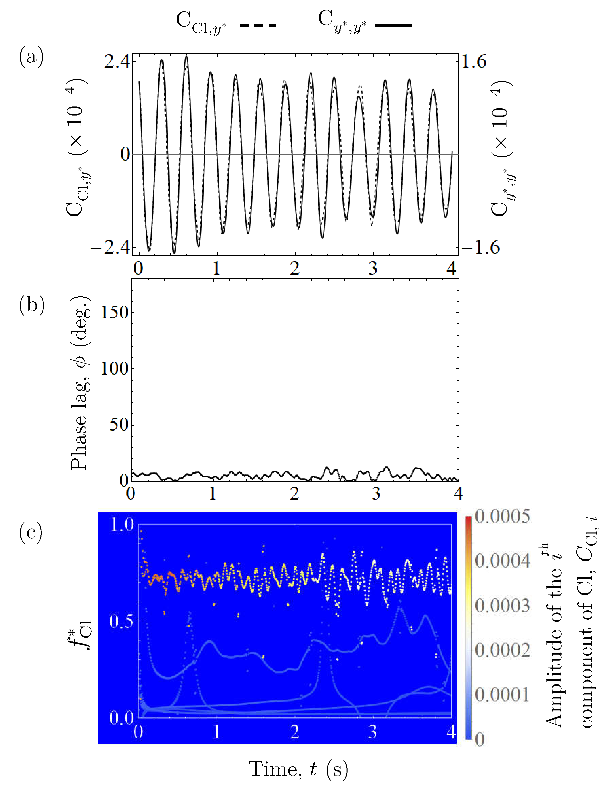
\includegraphics[width=0.5\textwidth]{figs/figure12}
  \caption{Temporal analysis of the lift coefficient and normalised cylinder displacement signal at $\ured = 4.5$. We show $\cclys$ and $\cclys$ side by side in Fig. \ref{fig:tempAnalysisKVIV}a, present the temporal evolution of the phase lag $\phi$ in Fig. \ref{fig:tempAnalysisKVIV}b and show the temporal evolution of the instantaneous frequency of the lift coefficient signal in Fig. \ref{fig:tempAnalysisKVIV}c.} \label{fig:tempAnalysisKVIV}
\end{figure}

Once we enter the upper branch of KVIV at  $\ured = 6.8$, $\phi$ jumps to approximately 110 deg. This jump in $\phi$ is characteristic of the transition to the upper branches as also observed by \citet{Maruai2018}, among others. Both $\cclys$ and $\cysys$ signals are visibly very periodic, and the dominant frequency band of Cl, is centred at $\approx 1$, as one can verify in Fig. \ref{fig:tempAnalysisUpper}c.

\begin{figure}
  \centering
  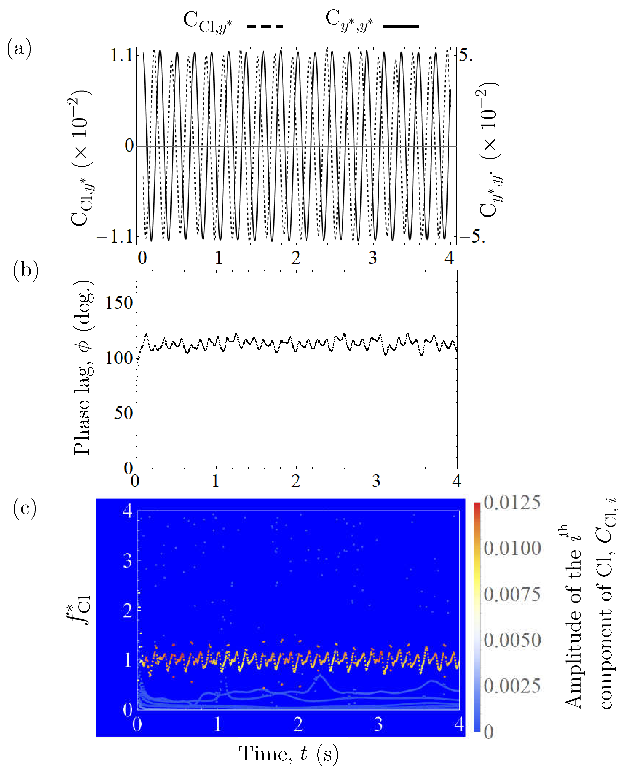
\includegraphics[width=0.5\textwidth]{figs/figure13}
  \caption{Temporal analysis of the lift coefficient and normalised cylinder displacement signal at $\ured = 6.8$. We show $\cclys$ and $\cysys$ side by side in Fig. \ref{fig:tempAnalysisUpper}a, present the temporal evolution of the phase lag $\phi$ in Fig. \ref{fig:tempAnalysisUpper}b and show the temporal evolution of the instantaneous frequency of the lift coefficient signal in Fig. \ref{fig:tempAnalysisUpper}c.} \label{fig:tempAnalysisUpper}
\end{figure}

As we increase $\ured$ even further up to $\ured = \ursi$, we see a similar trend for all $\ured = 9.1, 11.4, 13.6$ examined: $\cysys$ and $\cclys$ are both qualitatively very periodic. Their phase lags are very close to $180$ deg., and the dominant Cl frequency bands exhibit a time-averaged value that increases linearly with respect to $\ured$, in a manner that the Strouhal number of Cl is always $\approx 0.16$ on average. We present the representative case of $\ured = \ursi$ in Fig. \ref{fig:tempAnalysisLower}. Note how $\phi$ in this range of $\ured$ varies much less with respect to time, compared to $\phi$ at $\ured = \urth$, and the dominant frequency band of Cl is much narrower compared to the dominant frequency band at $\ured = \urth$, indicating a highly periodic and self-similar oscillation of lift.

\begin{figure}
  \centering
  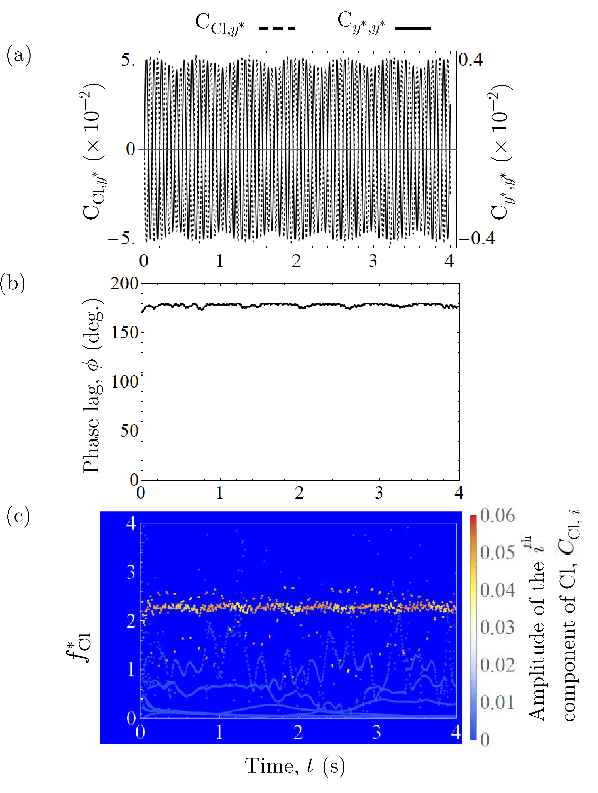
\includegraphics[width=0.5\textwidth]{figs/figure14}
  \caption{Temporal analysis of the lift coefficient and normalised cylinder displacement signal at $\ured = \ursi$. We show $\cclys$ and $\cysys$ side by side in Fig. \ref{fig:tempAnalysisLower}a, present the temporal evolution of the phase lag $\phi$ in Fig. \ref{fig:tempAnalysisLower}b and show the temporal evolution of the instantaneous frequency of the lift coefficient signal in Fig. \ref{fig:tempAnalysisLower}c.} \label{fig:tempAnalysisLower}
\end{figure}

\subsection{Transition to SVIV $\left (\urse \leq \ured \leq \urei \right )$} \label{ssec:transSVIV}
Previously in the $\ured \leq \ursi$ range, we observed that the temporal profile of both Cl and  $\ystr$ are very similar to each other, except that Cl leads $\ystr$ by a certain amount. This similarity in profile supports the assertion that the vibration within $\ured \leq \ursi$ is driven exclusively by the shedding of Karman vortices, which brings the onset of the alternating lift. Analogously, one might expect a similar profile between Cl and $\ystr$ when streamwise vortices drive the vibration. However, this does not seem to be the case.

Once we reach $\ured = 15.9$, we observe that it has become difficult to argue that the profile of $\ystr$ is just a lagged version of the profile of Cl. This is shown in Fig. \ref{fig:tempEvoCompare}a, with the enlarged version in Fig. \ref{fig:tempEvoCompare}b. The profile of Cl looks like the result of several signals in superposition, which one can almost distinguish from the presence of two types of maxima at two different amplitude heights. We put a red dashed line and a red dashed-dot line in Fig. \ref{fig:tempEvoCompare}b as visual cues indicating the two amplitude heights. Decomposing the lift coefficient signal using EEMD reveals partial evidence supporting the compound signal hypothesis.

\begin{figure}
  \centering
  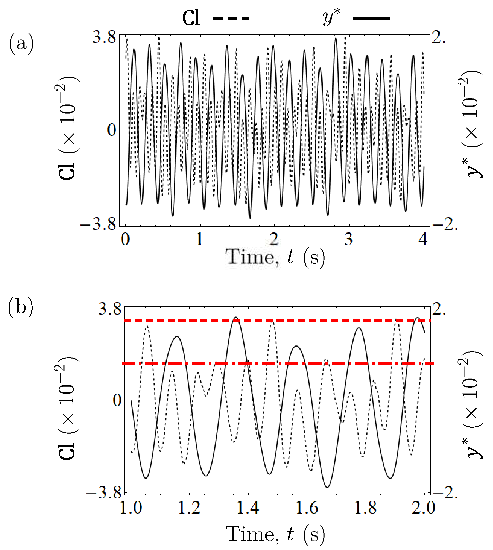
\includegraphics[width=0.4\textwidth]{figs/figure15}
  \caption{Temporal evolution of $\ystr$ and Cl at $\ured 15.9$. Figure \ref{fig:tempEvoCompare}b shows an enlarged view of Fig. \ref{fig:tempEvoCompare}a. We can barely spot semblance of two signals with different amplitudes superimposed in the Cl signal in Fig. \ref{fig:tempEvoCompare}b.} \label{fig:tempEvoCompare}
\end{figure}

Once we have decomposed the signal using EEMD, we replot Fig. \ref{fig:tempEvoCompare}a using $\cclys$ and $\cysys$ in Fig. \ref{fig:tempAnalysisTransition}a. One can clearly see that the part of Cl signal responsible for driving the vibration at  $\ured = 15.9$ is embedded in the original Cl signal (Fig. \ref{fig:tempAnalysisTransition}a), and decomposition via EEMD managed to recover this signal, which leads $\cysys$ by approximately 150 deg. on average, throughout the whole observation time (Fig. \ref{fig:tempAnalysisTransition}b). This decline from $\phi \approx 180$ deg. at reduced velocities $\urfo \leq \ured \leq \ursi$, to $\phi \approx 150$ deg. at $\ured = \urse$ is quite sizeable, suggesting a fundamental change in flow dynamics, particularly in terms of vortical structure. Another notable change is the increased temporal variation in $\phi$ from its time-averaged value, in contrast to the evolution of $\phi$ in the range $\urfo \leq \ured \leq \ursi$, which has very little jitter throughout the observation time.

\begin{figure}
  \centering
  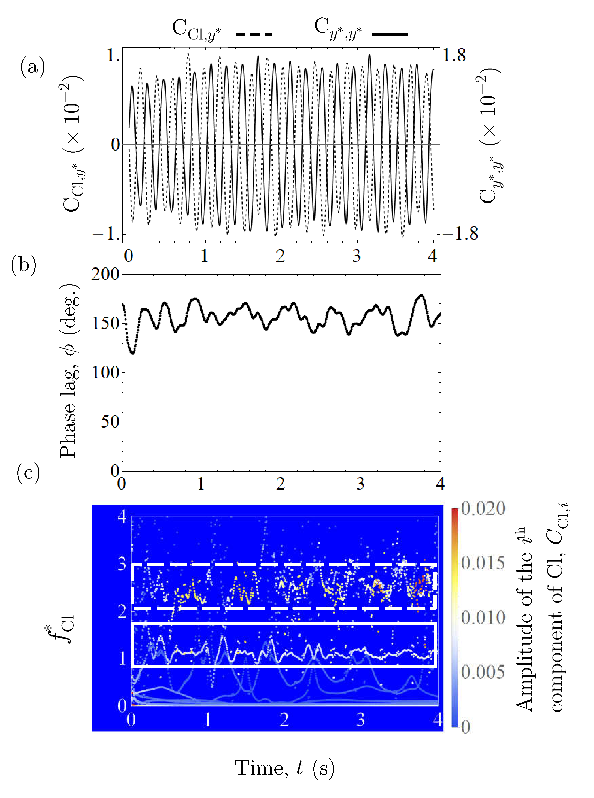
\includegraphics[width=0.45\textwidth]{figs/figure16}
  \caption{Temporal analysis of the lift coefficient and normalised cylinder displacement signal at $\ured = 15.9$. We show $\cclystr$ and $\cysys$ side by side in Fig. \ref{fig:tempAnalysisTransition}a, present the temporal evolution of the phase lag $\phi$ in Fig. \ref{fig:tempAnalysisTransition}b and show the temporal evolution of the instantaneous frequency of Cl in Fig. \ref{fig:tempAnalysisTransition}c.}
  \label{fig:tempAnalysisTransition}
\end{figure}

Inspecting the HHT spectrogram in Fig. \ref{fig:tempAnalysisTransition}c reveals two dominant bands in the frequency domain. The first one, marked with a white continuous rectangular box, is the instantaneous frequency for the IMF component of lift shown in Fig. \ref{fig:tempAnalysisTransition}a, and its mean frequency lies close to the natural frequency of the system ($\fclstr \approx 1$). There is; however, a second band of the frequency with nearly similar amplitude around $\fclstr \approx 3.3$, marked with a white dashed rectangular box. Computing the Strouhal number from this frequency returns a value of $\st = 0.20$, which is very close to the Strouhal number for Karman vortices as predicted by Eq. \ref{eq:karmanSheddingFreq} at the Reynolds number equivalent to $\ured = 15.9$, which is $\re = 7.9 \times 10^{3}$. We thus attribute this second band of frequency as being the footprint left by the shedding of Karman vortices, and the first band as the result of streamwise vortex shedding. Through visual inspection of Fig. \ref{fig:tempAnalysisTransition}c, both of these dominant frequency bands are markedly wider and the individual values are more scattered from their time-averaged values than any of their counterparts within $\ured \leq \ursi$.

The knowledge that Karman vortices continue to exist and shed from a cruciform structure during SVIV is not new in the literature. However, this is the first time the lift signal from a cruciform structure undergoing SVIV has been subjected to EEMD, revealing the signature of the two dominant vortical structures regulating the flow around the cruciform. Although the amplitude size of the instantaneous frequency band due to Karman vortex is comparable to the streamwise vortex, the reason why the cylinder resists locking into its frequency is perhaps that its frequency too distant from the natural frequency of the system $\fn$. The shedding frequency of the streamwise vortex is much closer to $\fn$ and is thus preferred by the cylinder.

We consider the transition to SVIV to be complete at $\ured = 18.2$, when the time-averaged phase lag drops further to $\approx 20$ deg. Figure \ref{fig:tempAnalysisStableInitialBranch}a and \ref{fig:tempAnalysisStableInitialBranch}b documents this observation. The instantaneous phase lag is observed to slip through 360 deg. a little past the two second (\SI{2}{\second}) time stamp. By inspecting Fig. \ref{fig:tempAnalysisStableInitialBranch}a, we found that a little past \SI{2}{\second} is when distortions in the periodicity of $\cclys$ occur. The slipping through 360 deg. was also observed by \citet{Khalak1999} in their work on KVIV, highlighting the quasi-periodic nature of the signal being analysed. There, the slip appeared in \citet{Khalak1999} at the initial branch of KVIV. The overall low value of $\phi$ ($\approx 20$ deg. for the whole observation time at $\ured = 18.2$), coupled with the presence of $\phi$ slippage are suggestive of the possibility for $\ured = 18.2$ being the initial branch of SVIV.

\begin{figure}
  \centering
  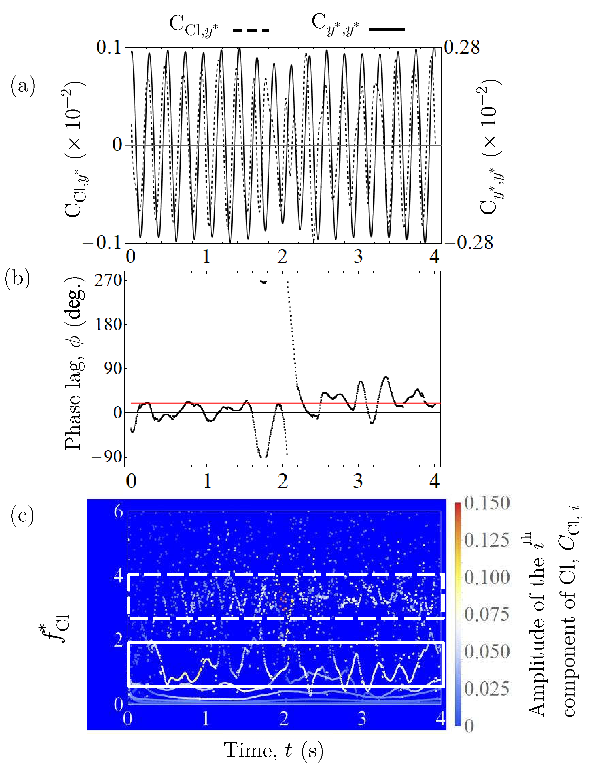
\includegraphics[width=0.47\textwidth]{figs/figure17}
  \caption{Temporal analysis of the lift coefficient and normalised cylinder displacement signal at $\ured = 18.2$. We show $\cclys$ and $\cysys$ side by side in Fig. \ref{fig:tempAnalysisStableInitialBranch}a, present the temporal evolution of the phase lag $\phi$ in Fig. \ref{fig:tempAnalysisStableInitialBranch}b and show the temporal evolution of the instantaneous frequency of Cl in Fig. \ref{fig:tempAnalysisStableInitialBranch}c.}
  \label{fig:tempAnalysisStableInitialBranch}
\end{figure}

\subsection{The stable SVIV regime $\left ( \ured \geq \urni \right )$} \label{ssec:svivRegime}
As $\ured$ is increased to 20.5, we can see a jump in $\phi$ from a mean value of approximately 20 deg. to about 120 deg., shown in Fig. \ref{fig:phaseAngle}a. The phase slippage discussed previously is also observed, indicating the quasi-periodic nature of the lift coefficient signal at this $\ured$. Incidentally, this quasi-periodicity seems to be the norm for the lift signals up to $\ured = 27.3$, as suggested by the phase slippages evident in Figs. \ref{fig:phaseAngle}b, c and d. The slippage only stops once $\ured$ reaches 29.5, suggesting a more periodic behaviour of the lift coefficient compared to its counterparts between $20.5 \leq \ured \leq 27.3$. Although the instantaneous phase between $20.5 \leq \ured \leq 27.3$ implies a quasi-periodic nature, their time-averaged values at each $\ured$ are contained in the narrow region $114 < \phi$ (deg.) $< 135$, as is the value for $\phi$ at $\ured = 29.5$. This observation that the time-averaged value of $\phi$ to only slowly vary with respect to $\ured$, once $\ured$ increases past 20.5, can be interpreted as the dominant flow structures settling into a stable form that becomes more resilient against external excitations. Based on this feature, we classified $20.5 \leq \ured \leq 29.5$ as the upper branch of SVIV.

\begin{figure}
  \centering
  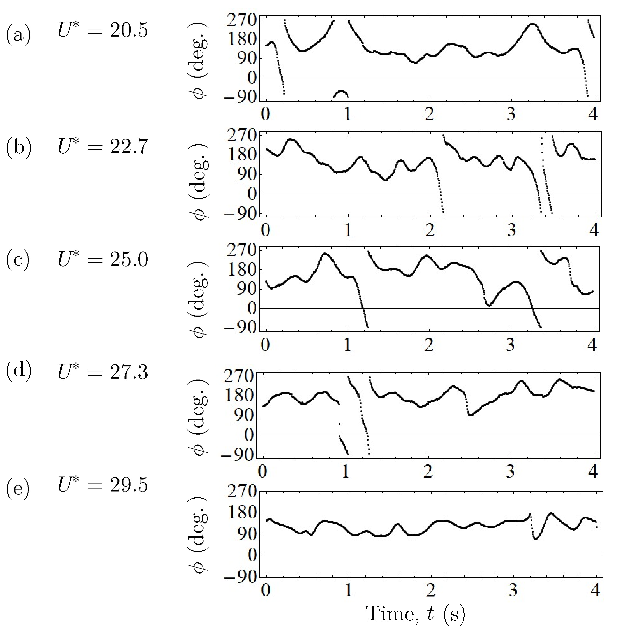
\includegraphics[width=0.45\textwidth]{figs/figure18}
  \caption{The instantaneous phase lag $\phi$ of $\cclys$ in the range $\urni \leq \ured \leq \urtt$. We can observe $\phi$ slipping through 360 deg. between $\urni \leq \ured \leq \urtv$, before disappearing at $\ured = \urtt$; an indication of improved stability and resilience of the vortical structure driving the vibration.}
  \label{fig:phaseAngle}
\end{figure}

The data on the evolution of $\phi$ allows us to construct a map of the ``branches'' of vibration modes observed in the range of $\ured$ that we studied. As the branches are mapped against $\ured$, we need a representative value of $\phi$ at each $\ured$. To achieve this, we took the time-averaged values of $\phi$, i.e. $\phim$, and plotted them against $\ured$ in Fig. \ref{fig:phaseAngleRegime}. The region A indicates the initial branch of  KVIV, where  $\phim$ is close to zero. Region B denotes the upper/lower branch of  KVIV, where the system experiences a jump from  $\phim \approx 0$ to greater than 110 deg. The value of $\phim$ settles very close to 180 deg. towards the end of this upper/lower branch.

\begin{figure}
  \centering
  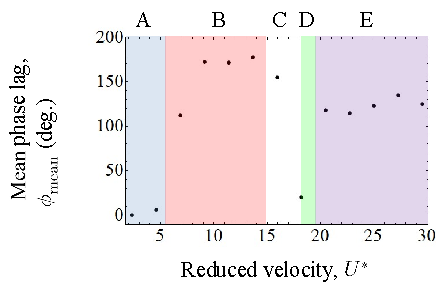
\includegraphics[width=0.37\textwidth]{figs/figure19}
  \caption{Vibration regimes identified during analysis of $\phi$. To capture the evolution of $\phi$ with respect to $\ured$, a representative value for $\phi$ at each $\ured$ must be selected. We chose to use the time-averaged $\phi$, $\phim$, as the representative value.}
  \label{fig:phaseAngleRegime}
\end{figure}

Then, $\phim$ experiences a slight drop from about one-sixth the value of $\phim$ in region B, as we enter region C, marking the start of the transition to the SVIV regime. Following this, the system undergoes a more sudden drop to $\phim \approx 20$ deg. at $\ured = 18.2$. This we designate as region D. Finally, in region E, we observe another jump in $\phim$ from $\phim \approx 20$ deg. in region D to approximately 120 deg. when $\ured \geq \urni$.


\section{Estimation of harnessable power} \label{sec:estimPow}
\subsection{Mathematical model for power estimation} \label{ssec:mathModel}
The mathematical model for harnessable power estimation in this study follows that which had been derived in \citet{Raghavanetal2007}. In these works, the authors mentioned that work done by the oscillating cylinder $\wcl$ during one cycle of oscillation $\tosc$ is as follows.

\begin{equation}
  \wcl = \int_{0}^{\tosc} \left ( \fl \cdot \dot{y} \right ) dt
  \label{eq:workCylinder}
\end{equation}

\noindent where both the lift $\fl$ and cylinder velocity $\dot{y}$ are both functions of time. Through several manipulations and simplifying assumptions \citep{Sun2016}, the power captured by the system can be written, using our parameters, as the fluid power

\begin{equation}
  \pfrms = \frac{1}{2} \rho \pi \cclrms U^{2} \fcyl \yrms D L \sin(\phi),
  \label{eq:rmsFluidPower}
\end{equation}

\noindent or the mechanical power

\begin{equation}
  \pmrms = 8 \pi^{3} \meff \zetatot \left (\yrms \fcyl \right )^{2} \fn.
  \label{eq:rmsMechPower}
\end{equation}

Here, $\pfrms$, $\pmrms$, $L$, $\cclrms$, $\zetatot$ and $\meff$ are the \rms{} of fluid power, \rms{} of mechanical power, length of the circular cylinder, characteristic \rms{} of lift amplitude, total damping coefficient, and the system effective mass respectively. We use $\cclys$ to represent $\cclrms$ in Eq. \ref{eq:rmsFluidPower}. We choose to use \rms{} (parameters with subscript RMS) quantities in Eq. \ref{eq:workCylinder} instead of the maximum values like the original authors because that may lead to a misunderstanding that the maximum value is sustained throughout the observation window. This obviously is not always the case in our study, especially once the system transits into the SVIV regime. Recall that the time series analysis of $\ystr\left( t \right)$ and $\text{Cl}\left( t \right)$ in \S\ref{ssec:ampResp} revealed that there is a degree of intermittency in both signals that cannot be overlooked at certain ranges of $\ured$. Using the \rms{} value allows us to partially take this into account in the estimation of harnessable power.

Figure \ref{fig:powerComparison} shows the comparison between power estimated from our experiment and numerical results, with the experimental results of \citet{Nguyen2012} and the direct power measurement of \citet{Koide2013}. Only the value for $\pmrms$ is computed from our experimental results due to the absence of lift data. Our numerical results have both lift and cylinder displacement data, and hence, we calculated both $\pfrms$ and $\pmrms$. We estimated the power from the experimental results of \citet{Nguyen2012} by interpolating missing data points in both their amplitude and frequency responses to compute the value of $\pmrms$ at a given value of $\ured$. The direct power measurement by \citet{Koide2013} was done by connecting the elastic support of the cylinder to a coil. The coil moves with the cylinder, thus creating a relative pistoning motion against a fixed magnet and produces an alternating current.

\begin{figure}
  \centering
  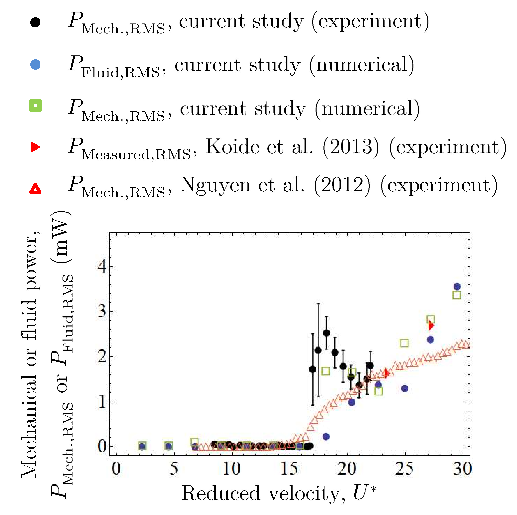
\includegraphics[width=0.4\textwidth]{figs/figure20}
  \caption{Estimated \rms{} of mechanical power $\pmrms$, fluid power $\pfrms$, or both, of our experimental and numerical results, compared with results of similar studies in the literature. The fluid power $\pfrms$ is calculated only from the results of our numerical study as the others did not measure lift.}
  \label{fig:powerComparison}
\end{figure}


\begin{figure}
  \centering
  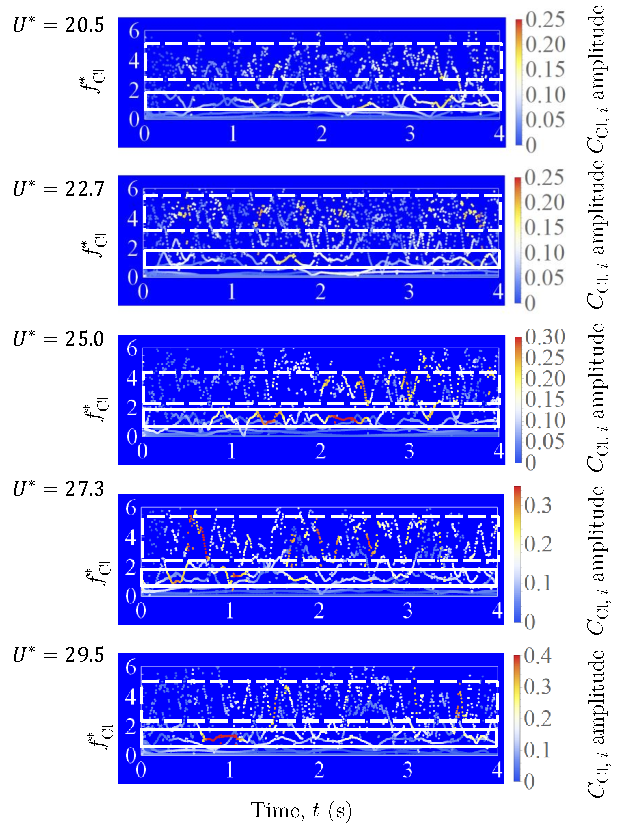
\includegraphics[width=0.47\textwidth]{figs/figure21}
  \caption{The instantaneous frequency of the lift signal between $\urni \leq \ured \leq \urtt$. The white, solid boxes enclose the IMF component of Cl due to the shedding of the streamwise vortex, while the dashed, white boxes enclose the IMF component due to the shedding of Karman vortex. Through visual inspection, we can see how the degree of dispersion (i.e., height of the box) in the instantaneous frequency of the ``Karman component'' of lift is about twice that of the ``streamwise component'' of lift.}
  \label{fig:instantLiftFreq}
\end{figure}

The estimated power in the KVIV regime $\ured \leq \urse$ produces power only in the order of \si{\micro\watt}, which is relatively insignificant in contrast to the magnitude of power produced in the SVIV regime (mW). In the region $\urei \leq \ured \leq \urte$, $\pmrms$ for our experiment and numerical work exhibits a similar trend where we observed a sudden jump in power output, followed by a gradual decrease. This gradual decrease can be attributed to the increased turbulence level right after the onset of SVIV that imposes a degree of intermittency to the normalised cylinder displacement signal, $\ystr$. For $\pfrms$, however, the quantity exhibits a monotonic increase in the range $\urei \leq \ured \leq \urte$. We only observe a dip in $\pfrms$ at $\ured = \urel$, suggesting an increase in intermittency of $\cclys$ at this $\ured$. In the experimental work of \citet{Nguyen2012}, $\pmrms$ only experiences a monotonic increase in the region $\urei \leq \ured \leq \urte$. This decidedly different response of the system compared to ours most likely stem from the difference in the actual cruciform used by \citet{Nguyen2012}. They used two circular cylinders of diameter \SI{10}{\milli\metre} as their cruciform, whereas we used a circular cylinder - strip plate in both our experiments and numerical work. There are no data from the direct power measurement of \citet{Koide2013} to compare with within $\urei \leq \ured \leq \urte$.

In the range $\urel \leq \ured \leq \urtt$, we find a reasonably good agreement between the trend found in all data compared: they increase monotonically with respect to $\ured$. Although the value of our $\pfrms$ falls quite notably below the value of $\pmrms$ at $\ured = \urel$, other values of $\pfrms$, $\pmrms$ from our numerical results and the direct power measurements by \citet{Koide2013} agree well within $\urtv \leq \ured \leq \urtt$. The only set of power data that consistently falls quite a distance below the others is the $\pmrms$ estimated from the experimental data of \citet{Nguyen2012}, which again, is most probably due to the difference in the actual geometry of the cruciform used in their investigation.


\subsection{Possibility for increasing fluid power, $\pfrms$} \label{ssec:possIncrease}
Recall in Fig. \ref{fig:powerComparison} that although $\pfrms$ is computed according to Eq. \ref{eq:rmsFluidPower}, which uses $\cclrms$ instead of the actual \rms{} amplitude of lift ($\clrms$), the resulting power estimate does not result in a trend that is totally different from the trend found in the other datasets. Furthermore, except for $\pmrms$ estimated from the experimental data of \citet{Nguyen2012}, the values of $\pfrms$ are in fairly good agreement with other data that it is compared against at high $\ured$ ($\ured = \urtv$ and $\urtt$). We see this is an indication that the lift component selected for use in computation of $\pfrms$ is an arguably faithful representation of the force driving the motion of the cylinder. This suggests that the motion of the cylinder, once it enters the SVIV regime, is driven only by one component, and not the totality, of the lift force. This component -- that has a time-averaged frequency close to the natural frequency of the system, $\fn$ -- is the ``streamwise component'' of lift.

Another significant IMF component of the lift force in the SVIV regime is the component whose mean frequency is close to the Karman frequency of vortex shedding, as explained in \S\ref{ssec:transSVIV}. This Karman component of lift has a similar amplitude size as the streamwise component of lift, as evidenced in Fig. \ref{fig:instantLiftFreq}, and as such is also a dominant component of lift. The Karman components are marked with a dashed, white box, and the streamwise components are marked with a solid, white box, following the convention in Figs. \ref{fig:tempAnalysisKVIV}, \ref{fig:tempAnalysisUpper}, \ref{fig:tempAnalysisLower}, \ref{fig:tempAnalysisTransition} and \ref{fig:tempAnalysisStableInitialBranch}. However, the Karman component fails to affect the cylinder vibration like the streamwise component most probably due to the large difference between the mean frequency of the Karman component and the natural frequency of the system, $\fn$.  The streamwise component has a mean frequency close to $\fn$ and is hence able to synchronise with the vibration of the cylinder, producing a sizeable amplitude response.

\begin{figure}
  \centering
  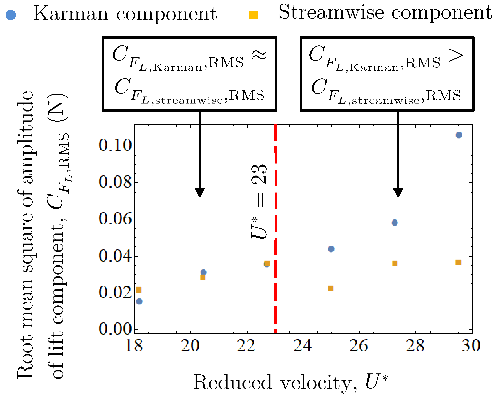
\includegraphics[width=0.43\textwidth]{figs/figure22}
  \caption{Evolution of the \rms{} amplitude of two dominant lift components due to Karman ($\cflkrms$) and streamwise ($\cflsrms$) vortices with respect to $\ured$. The region $\urei \leq \ured \leq \urte$ exhibits similar magnitude for both the Karman and streamwise components of lift. On the other hand, the magnitude of amplitude for the Karman component while the region $\urel \leq \ured \leq \urtt$ is almost always twice that of the streamwise component.}
  \label{fig:karmanStreamwiseComponents}
\end{figure}

Figure \ref{fig:karmanStreamwiseComponents} shows the \rms{} amplitude of the Karman and streamwise components of lift in the SVIV regime $\ured \geq \urei$. Between $\urei \leq \ured \leq \urte$, the magnitude of the Karman and streamwise components are nearly equal. However, once we exceed $\ured = \urte$, Fig. \ref{fig:karmanStreamwiseComponents} shows that the contribution to the \rms{} amplitude of total lift by the Karman component is on average twice the contribution of the streamwise component. Having such a significant contribution towards the \rms{} amplitude of total lift implies that there is a significant portion of energy from the free stream being used to energise the Karman vortex structure in the flow. Let us assume a hypothetical situation where we can transfer the contribution by the Karman component to the streamwise component of lift. In other words, consider the situation where we can completely redirect the energy from the Karman to the streamwise vortex. Then, the value for $\cclrms$ in Eq. \ref{eq:rmsFluidPower} will increase close to a factor of 2 when $\urei \leq \ured \leq \urte$, and close to a factor of 3 when $\urel \leq \ured \leq \urtt$. This increase in $\cclrms$ will lead to the scaling of $\pfrms$ by the same factor, keeping the other parameters in Eq. \ref{eq:rmsFluidPower} constant. This exercise demonstrates the room for improvement possible for $\pfrms$ in future developments of cruciform energy harvesters.

\color{blue}
One possible method of improving $\pfrms$ is by implementing a modified version of the cruciform that is able to enforce the dominance of the vortical structure that is able to lock into $\fn$ - which in Fig. \ref{fig:karmanStreamwiseComponents} is the streamwise vortex - against the vortical structures that do not, i.e., the Karman vortices. We will outline such a method in our future work.
\color{black}

\section{Conclusions} \label{sec:conclusions}
In this study, we numerically investigated the temporal evolution of the lift coefficient and cylinder displacement signals of an elastically supported cruciform system in the range $1.1 \times 10^{3} < \re < 14.6 \times 10^{3}$, or $\uron < \ured < \urtt$. Our circular cylinder diameter is \SI{10}{\milli\metre} and the natural frequency of the system is \SI{4.4}{\hertz}. Validation of key numerical results was made experimentally in a custom-built open flow channel, using a cruciform system whose parameters were tuned as close as possible to the quantities used in the numerical study. Decomposing the lift coefficient signal in the SVIV regime ($\urse \leq \ured \leq \urtt$) using EEMD allows us to see that the complexity of the lift coefficient signal as being caused by the superpositioning of two dominant components of lift. One due to the shedding of Karman and the other due to the shedding of streamwise vortices. The former has a frequency close to the vortex shedding frequency of Karman vortex from a smooth, isolated circular cylinder, while the latter has a mean frequency close to $\fn$. Application of the Hilbert-Huang transform on the dominant component of cylinder displacement -- and the component of lift most correlated to it -- allows for the computation of the instantaneous phase lag between lift and cylinder displacement. The time-averaged phase lag revealed five ``branches'' of vibration, among which is the initial branch of SVIV at $\ured = \urei$, which has never been identified before in the literature. We also computed the instantaneous frequency of the lift coefficient, thus revealing the loss of periodicity and self-similarity in the lift coefficient signal as the system enters the SVIV regime. Estimation of power from our results show that the \rms{} mechanical and fluid power computed from our experimental and numerical work agree to varying degrees depending on $\ured$ with data from similar studies in the literature. Finally, we estimated that the \rms{} fluid power can potentially be increased close to a factor of 2 within $\urei \leq \ured \leq \urte$ and close to a factor of 3 when $\urel \leq \ured \leq \urtt$. We base this estimation on the premise of redirecting the contribution to the \rms{} amplitude of total lift from Karman vortex shedding, towards the streamwise component of lift alone.

%\appendix
%\section{Appendix}
%Appendix sections are coded under \verb+\appendix+.
%
%\verb+\printcredits+ command is used after appendix sections to list 
%author credit taxonomy contribution roles tagged using \verb+\credit+ 
%in frontmatter.
%

\printcredits

%% Loading bibliography style file
%\bibliographystyle{model1-num-names}
\bibliographystyle{cas-model2-names}

% Loading bibliography database
\bibliography{references}


%\vskip3pt

%\bio{}
%Author biography without author photo.
%Author biography. Author biography. Author biography.
%Author biography. Author biography. Author biography.
%Author biography. Author biography. Author biography.
%Author biography. Author biography. Author biography.
%Author biography. Author biography. Author biography.
%Author biography. Author biography. Author biography.
%Author biography. Author biography. Author biography.
%Author biography. Author biography. Author biography.
%Author biography. Author biography. Author biography.
%\endbio
%
%\bio{figs/pic1}
%Author biography with author photo.
%Author biography. Author biography. Author biography.
%Author biography. Author biography. Author biography.
%Author biography. Author biography. Author biography.
%Author biography. Author biography. Author biography.
%Author biography. Author biography. Author biography.
%Author biography. Author biography. Author biography.
%Author biography. Author biography. Author biography.
%Author biography. Author biography. Author biography.
%Author biography. Author biography. Author biography.
%\endbio
%
%\bio{figs/pic1}
%Author biography with author photo.
%Author biography. Author biography. Author biography.
%Author biography. Author biography. Author biography.
%Author biography. Author biography. Author biography.
%Author biography. Author biography. Author biography.
%\endbio

\end{document}
